\chapter{Instrumentation and experimental setup for SAXS measurements}
\label{chap:experimental_setup}

\section{BESSY II}

\subsubsection{Electron Accelerator}

The electron beam creates the free electrons: a hot thermionic cathode emits electrons which are accelerated with a high voltage to the anode until they reach energies up to 70 keV. The free electrons are transferred to a linear pre-accelerator which accelerates electrons to relativistic velocities up to 0.99c via an electric field. The electrons are then inserted into the microtron, which further accelerates the electrons to 50 MeV, at which point they are injected into the synchrotron. The acceleration process takes 50 ms and can be repeated with a repetition rate of 10 Hz with successive injection of electrons. Inside the synchrotron, a set of magnets are disposed in such a way as to lead the electrons in circular trajectories, whilst high frequency (HF) resonators in linear paths of the synchrotron, temporally coupled with the magnets, further accelerate the electrons to 1.72 GeV 18 .

\subsubsection{Storage ring}

The threshold energy is reached when a high electron flux with high temporal stability is achieved. At this point the electrons are injected into the storage ring, where bending magnets are implemented to maintain the circular trajectory of the electron, as shown in Figure \ref{fig:BessyScheme}. The storage ring has a circumference of 240 meters and the successive injection of electrons from the synchrotron leads to currents of approximately 290 mA in the initial stage (after injection).

\begin{figure}%[htbp]
	\centering
		\resizebox{0.4\linewidth}{!}{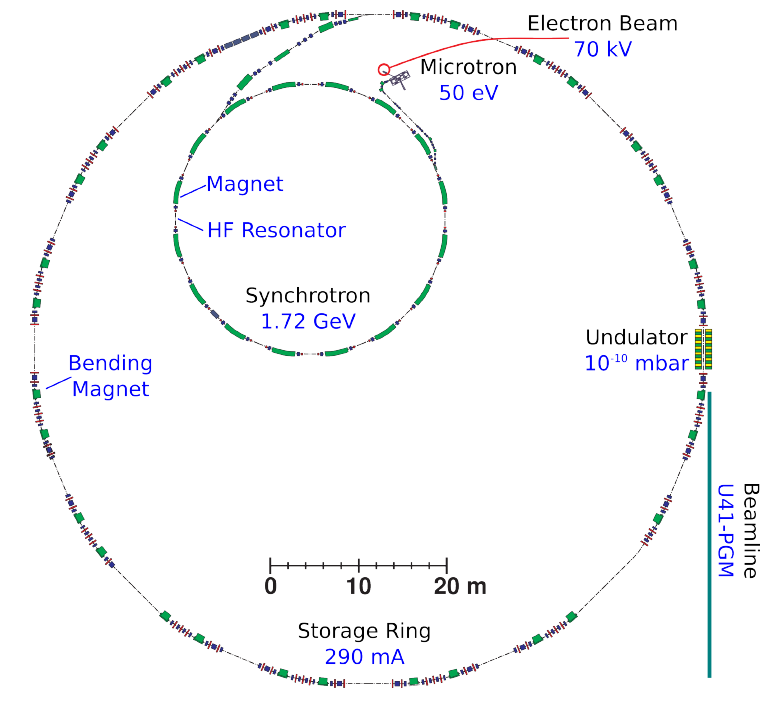
\includegraphics{Figures/BessyScheme.png}}
		\caption{A scheme of BESSY II. From the master thesis.}
		\label{fig:BessyScheme}
\end{figure}

\subsection{Insertion devices}

\subsubsection{Bending magent and bremsstrahlung radiation}
It is known that relativistic electrons lose kinetic energy due to the Bremsstrahlung process\citep{blumenthal_bremsstrahlung_1970} when they are accelerated or deaccelerated. This energy loss in the storage ring is compensated by high frequency resonators situated on a short linear section. In the case of a storage ring with circular shape, the electron bunches are accelerated radially (a perp v) and emit synchrotron radiation tangentially to the bunch trajectory. The power emitted


Total radiated power:
\begin{equation}
        P=\frac{e^2\gamma^4}{6\pi\epsilon_0c}\left( \dot{\beta}^2 + \frac{(\dot{\vec{\beta}} \cdot \vec{\beta})^2}{1-\beta^2} \right)
\end{equation}
where $\vec{\beta}=\frac{\vec{v}}{c}$ and $\gamma=\frac{1}{\sqrt{1-\beta^2}}$ is the Lorentz factor.

If the trajectory of the electrons and the acceleration are perpendicular, for circular particle trajectories:
\begin{equation}
        P_{a \bot v}=\frac{e^2\gamma^4}{6\pi\epsilon_0c}\dot{\beta}^2=\frac{e^2\gamma^4a^2}{6\pi\epsilon_0c^3}
\end{equation}

\subsubsection{Other devices: Wigglers and undulators}

 High photon flux
 
The energy range is also different.

Deflection parameter $K$. The difference between both types of devices is K. Normally you can vary K by increasing the space in the magnetic field (gap).

\begin{equation}
        K=\frac{eB_0\lambda_0}{m_0 2\pi c}
\end{equation}


\section{FCM Beamline}

Talk a little bit about design with mirrors and collimation

focused on the sample and collimated into a \(0.5\) mm circular spot by Ge pinholes situated between the sample and the monochromator

\begin{figure}%[htbp]
	\centering
		\resizebox{0.8\linewidth}{!}{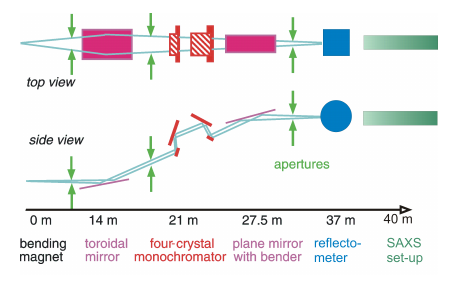
\includegraphics{Figures/FCMScheme.png}}
		\caption{A scheme of BESSY II. From the master thesis.}
		\label{fig:FCMScheme}
\end{figure}

\begin{figure}%[htbp]
	\centering
		\resizebox{0.7\linewidth}{!}{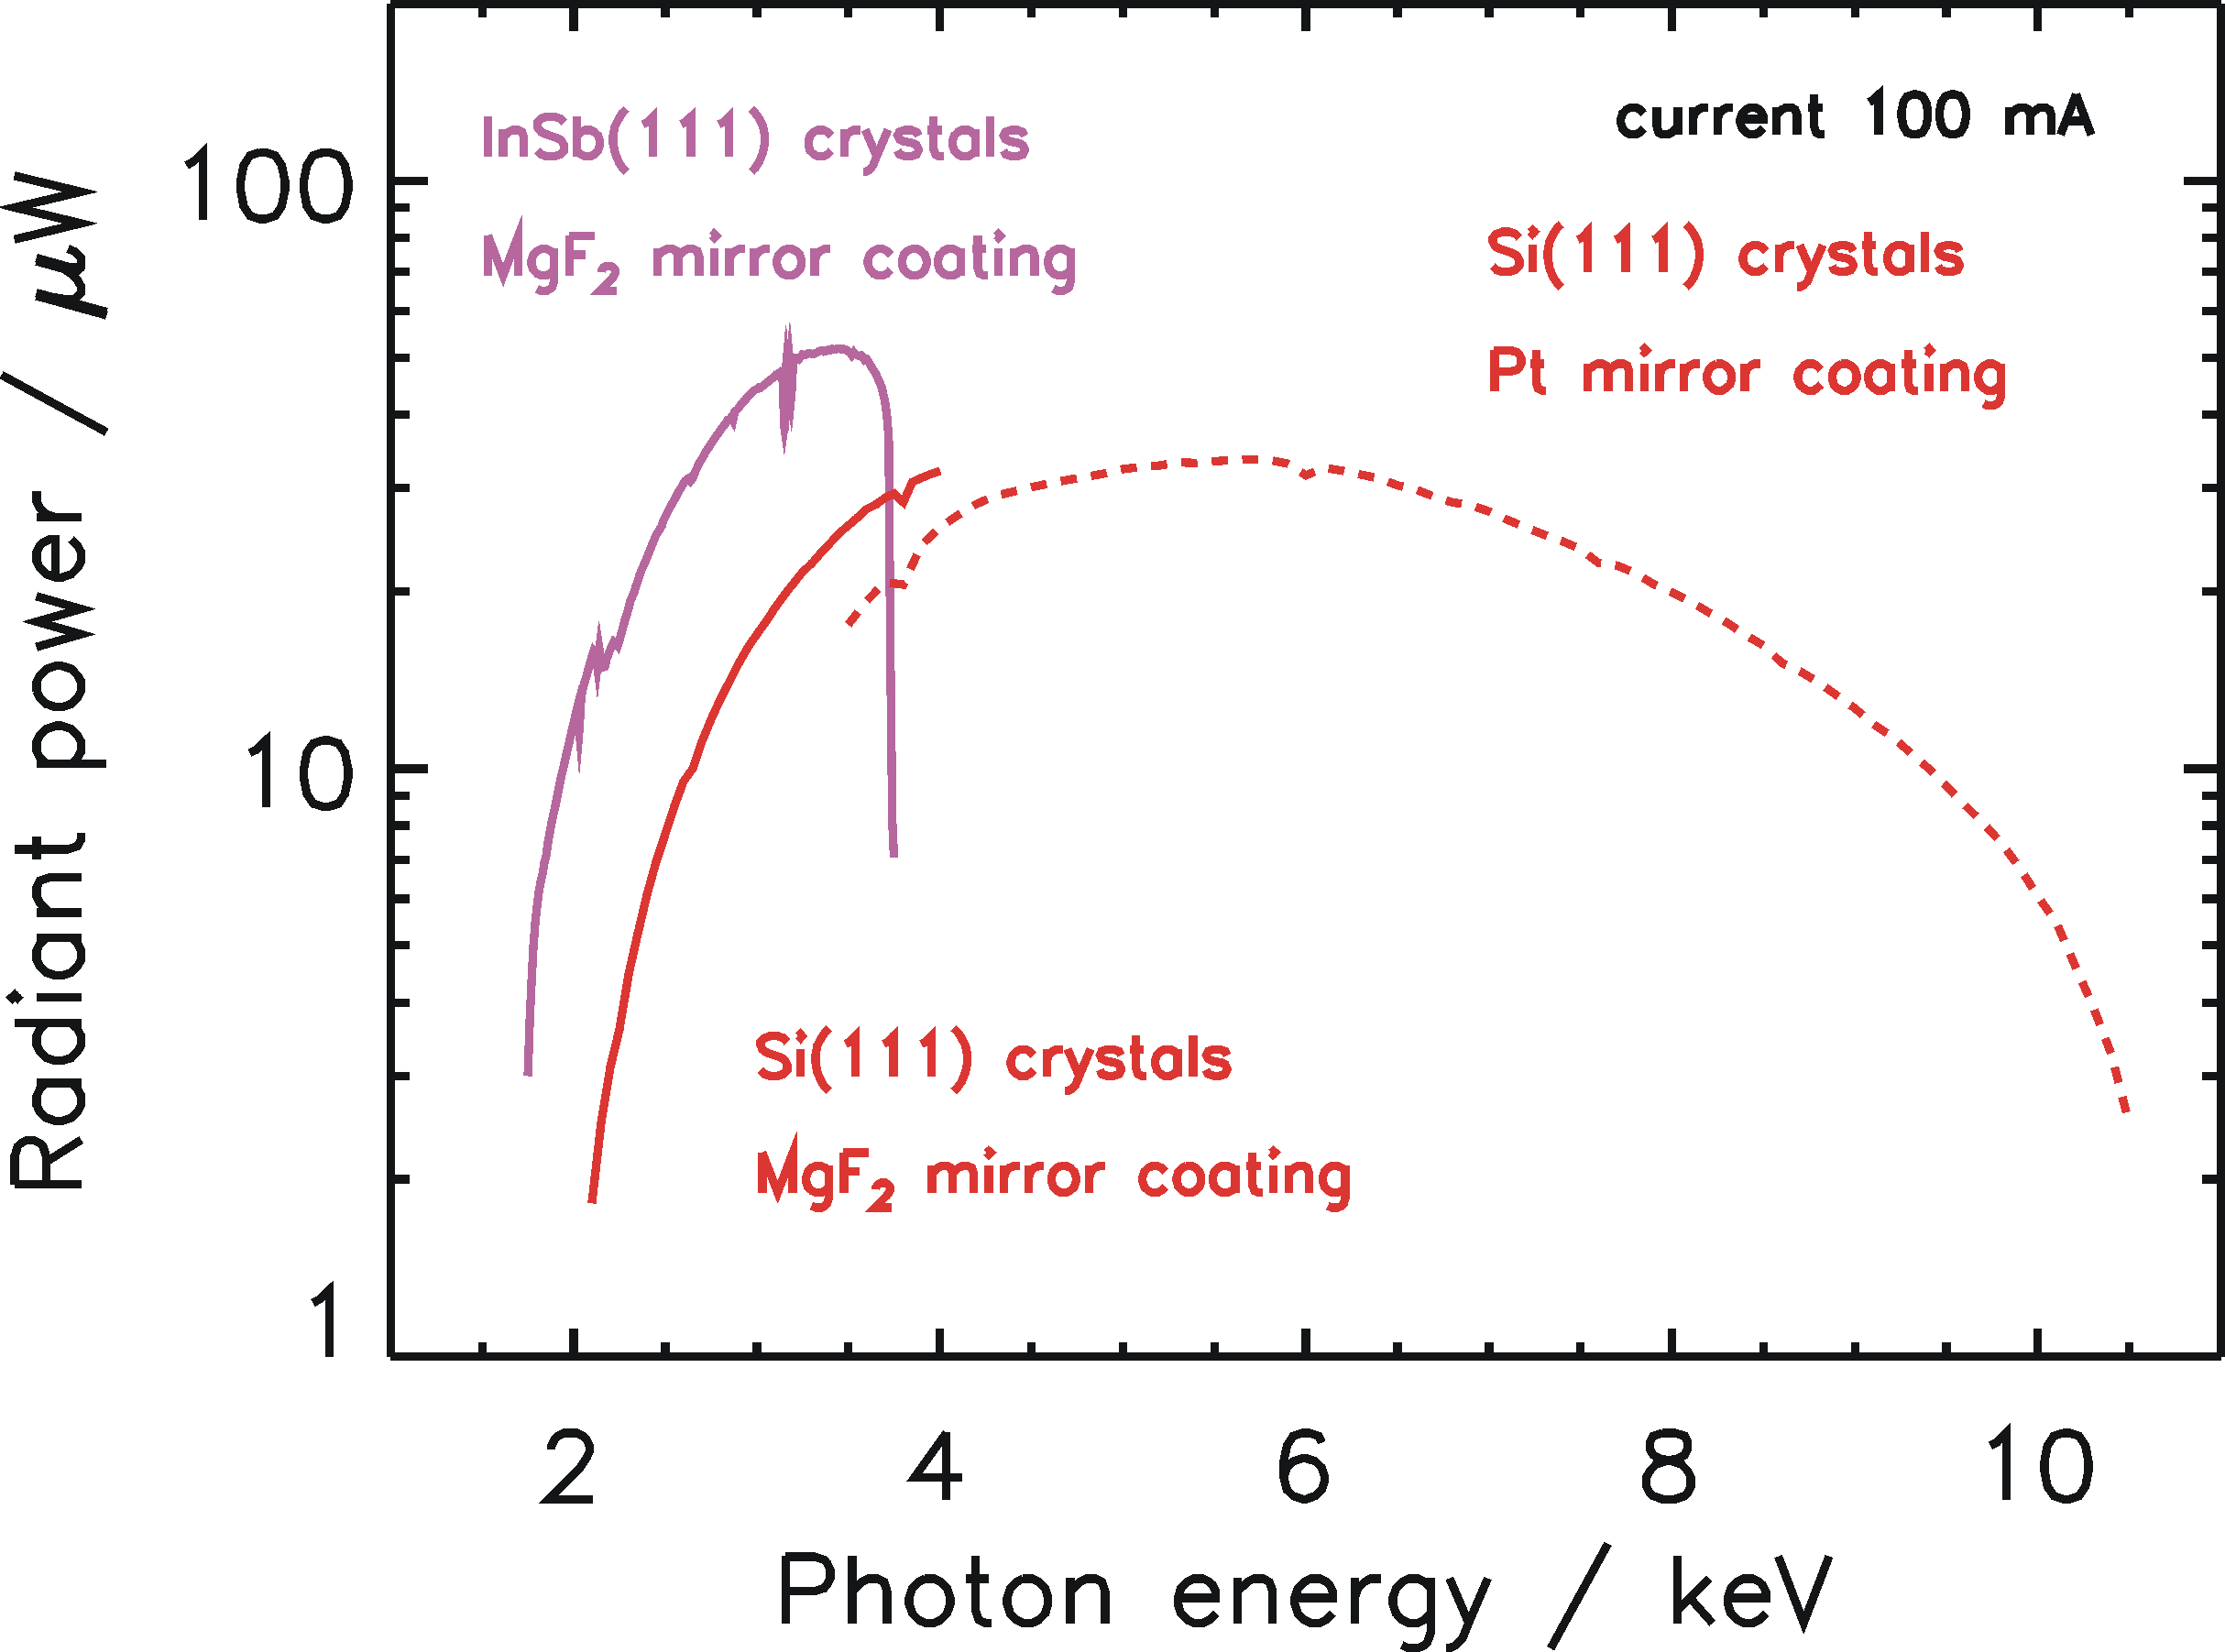
\includegraphics{Figures/FCMBeamlineFlux.png}}
		\caption{Typical flux scheme of the FCM Beamline}
		\label{fig:FCMBeamlineFlux}
\end{figure}

\subsection{Four-crystal monochromator}
\label{sec:fcm}

energy resolving power \( E/\Delta E \) of \( 10^4 \)

Energy resolution

Typical flux on the sample

Difference between Si and InSb

Beam size on the sample, divergence (talk to Mika)

The Four Crystal Monochromator consists of two times four crystals, where one set consists of InSb(111) and one of Si(111). The arrangement of the four crystals (see fig. 3.2) per set provides a stable beam position behind the monochromator, when changing the photon energy. This prevents a time consuming realignment as well as a change of the measured sample area. In SAXS, this enables double-checking a measurement result by changing the q area without moving the sample or the detector.

In the energy range from 1.75 keV up to 10 keV, this monochromator provides a spectral purity of 10-4, for energies higher than 2.5 keV even 3x10-5 . Behind the FCM at 27.5 m distance from the dipole, a plane bendable mirror reflects the beam back to horizontal direction and collimates it in vertical direction. This mirror has two different coating areas (Pt and MgF2 ) to enable the different energy ranges (see fig. 3.3). The flux reached at the beamline for the different energies and the different setups of the monochromator is shown in fig. 3.3. A slit downstream of the plane mirror reduces the beam size. Behind this, a thin photodiode can be placed to measure the photon flux in transmission [55].


\subsection{Monitor diode: Flux monitor}

Continuous measurement of the incoming photon flux with a semitransparent silicon diode 8 $\mu$m thick. It can be used down until 3 keV approx.

Avoiding possible fluctuations on the flux. TopUp mode should improve this but still there are variation between 297 and 299 mA which are around 1$\%$

\subsection{Reflectometer in vacuum: NewRef}

goniometer allowing us to move with high precision

The rectangular capillary is placed in a sample holder which allows the movement with micrometer precision in the directions perpendicular to the incoming beam, as depicted in figure \ref{fig:DensityGradientCapillarySetup}.

About 10 m behind the monochromator, the UHV X-ray Reflectometer [53] is located as sample chamber. The pressure in the reflectometer can be reduced to 10-7 mbar. Additionally, it provides devices to move and tilt samples in all directions, which allows to place up to 15 SAXS sample capillaries at once, without the need of breaking the vacuum and re-evacuate the chamber for changing the sample. Another important feature consists in the diodes which can be placed in the beam and are used to record the actual flux hitting the sample and to measure the transmission of the sample at the actual photon energy. Both are parameters required for the analysis of SAXS data.


\subsubsection{Transmission measurements}

calibrated diodes, SYRES II???? Calibrated agains cryo-radiometer every 3 years.

To measure the total flux and sample transmission, photodiodes were used which were calibrated against a cryogenic electric substitution radiometer with a relative uncertainty of \( 1\,\% \) \cite{krumrey_high-accuracy_2001}.

very thick silicon diodes

around 0.5 $\%$ uncertainty

\section{SAXS Setup}

How do we measure small-angle x-ray scattering?

\subsection{Pilatus detector}
high dynamic range

noise free

A vacuum-compatible Pilatus 1 M hybrid pixel detector (Dectris Ltd, Baden, Switzerland) with a pixel size of $d = (172.1 \pm 0.2)$ $\mu$m collected the scattered X-ray photons

\subsubsection{Beam-stop}

In order to avoid saturation effects in the center

diode in beamstop to see variation of the transmission during the measurement

\subsection{HZB SAXS instrument}

A very capable setup providing a large range for the sample-detector distance, a high resolution and high dynamic range detector, and a vacuum of about 10-4 mbar between sample chamber and detector is the SAXS setup of the Helmholtz-Zentrum Berlin (HZB). The distance variability is provided by bellows which allow a travel range of about 2.3 m. Additionally, one of these bellows can be removed to further decrease the sample-detector distance.


Collaboration with HZB (the SAXS setup of the Helmholtz-Zentrum Berlin (HZB))

Continuos distance movement between 1.5 and 3.7 m (or so)

The distance variability is provided by bellows which allow a travel range of about 2.3 m. 

Possibility to extract the bellows (WAXS)

Which q-range are available for each distance and energy? Small table for high and low energy \ref{tab:qrange}

\begin{table}[]
\centering
\caption{$q$-range available for the different experimental setups at extreme conditions. \textcolor{red}{CHECK FOR TRUE VALUES}}
\label{tab:qrange}
\begin{tabular}{|l|c|c|}
\hline
              & \textbf{SAXS} & \textbf{WAXS} \\ \hline
Distance (mm) & 4540          & 700           \\ \hline
Energy (eV)   & 4000          & 10000         \\ \hline
$q_{min}$ (nm$^{-1}$)   & \textbf{0.015}         & 0.5           \\ \hline
$q_{max}$ (nm$^{-1}$)   & 0.56             & \textbf{7}             \\ \hline
\end{tabular}
\end{table}

\subsubsection{Calibration of the sample-detector distance}

In small-angle scattering experiments, it is crucial to know precisely the distance between the irradiated sample and the detector, in order to calibrate the momentum transfer $q$. Typically, a calibration standard material with a well-known crystal lattice parameter is employed, which produces well-defined diffraction rings in the low-angle region. A material extensively used is dry rat-tail tendon collagen, with a $d$-spacing of 650 \AA \citep{amenitsch_performance_1997}, corresponding to $q=0.097$ nm$^{-1}$. The degradation of this material upon prolonged radiation suggested the use of harder calibrants such as silver behenate (CH$_3$(CH$_2$)$_{20}$COO$\cdot$Ag) \citep{huang_x-ray_1993}.

AgBehe has a very narrow diffraction ring at $q=1.0763$ nm$^{-1}$, arising from a long-period spacing ($d_{001]}$) value of 58.36 \AA \citep{blanton_jcpdsinternational_1995}, although this value depends slightly on the synthesis. A deviation of 0.5 $\%$ in the diffraction peak position could be observed for different sample preparations. In order to increase the accuracy of the calibration, the sample-detector distance was determined by the detection of the scattering pattern of AgBehe at different positions of the HZB SAXS instrument, measured with the built-in 3 m long Heidenhain optical encoder with an uncertainty of 20 $\mu$m. By triangulating the radius of the diffraction ring to the source point, as depicted in figure \ref{fig:DistanceCalibrationSAXS}, the sample-detector distance is obtained in a traceable way.

\begin{figure}
	\centering
	        \subfloat[Distance Calibration]{\resizebox{0.44\linewidth}{!}{% GNUPLOT: LaTeX picture with Postscript
\begingroup
  \makeatletter
  \providecommand\color[2][]{%
    \GenericError{(gnuplot) \space\space\space\@spaces}{%
      Package color not loaded in conjunction with
      terminal option `colourtext'%
    }{See the gnuplot documentation for explanation.%
    }{Either use 'blacktext' in gnuplot or load the package
      color.sty in LaTeX.}%
    \renewcommand\color[2][]{}%
  }%
  \providecommand\includegraphics[2][]{%
    \GenericError{(gnuplot) \space\space\space\@spaces}{%
      Package graphicx or graphics not loaded%
    }{See the gnuplot documentation for explanation.%
    }{The gnuplot epslatex terminal needs graphicx.sty or graphics.sty.}%
    \renewcommand\includegraphics[2][]{}%
  }%
  \providecommand\rotatebox[2]{#2}%
  \@ifundefined{ifGPcolor}{%
    \newif\ifGPcolor
    \GPcolortrue
  }{}%
  \@ifundefined{ifGPblacktext}{%
    \newif\ifGPblacktext
    \GPblacktextfalse
  }{}%
  % define a \g@addto@macro without @ in the name:
  \let\gplgaddtomacro\g@addto@macro
  % define empty templates for all commands taking text:
  \gdef\gplbacktext{}%
  \gdef\gplfronttext{}%
  \makeatother
  \ifGPblacktext
    % no textcolor at all
    \def\colorrgb#1{}%
    \def\colorgray#1{}%
  \else
    % gray or color?
    \ifGPcolor
      \def\colorrgb#1{\color[rgb]{#1}}%
      \def\colorgray#1{\color[gray]{#1}}%
      \expandafter\def\csname LTw\endcsname{\color{white}}%
      \expandafter\def\csname LTb\endcsname{\color{black}}%
      \expandafter\def\csname LTa\endcsname{\color{black}}%
      \expandafter\def\csname LT0\endcsname{\color[rgb]{1,0,0}}%
      \expandafter\def\csname LT1\endcsname{\color[rgb]{0,1,0}}%
      \expandafter\def\csname LT2\endcsname{\color[rgb]{0,0,1}}%
      \expandafter\def\csname LT3\endcsname{\color[rgb]{1,0,1}}%
      \expandafter\def\csname LT4\endcsname{\color[rgb]{0,1,1}}%
      \expandafter\def\csname LT5\endcsname{\color[rgb]{1,1,0}}%
      \expandafter\def\csname LT6\endcsname{\color[rgb]{0,0,0}}%
      \expandafter\def\csname LT7\endcsname{\color[rgb]{1,0.3,0}}%
      \expandafter\def\csname LT8\endcsname{\color[rgb]{0.5,0.5,0.5}}%
    \else
      % gray
      \def\colorrgb#1{\color{black}}%
      \def\colorgray#1{\color[gray]{#1}}%
      \expandafter\def\csname LTw\endcsname{\color{white}}%
      \expandafter\def\csname LTb\endcsname{\color{black}}%
      \expandafter\def\csname LTa\endcsname{\color{black}}%
      \expandafter\def\csname LT0\endcsname{\color{black}}%
      \expandafter\def\csname LT1\endcsname{\color{black}}%
      \expandafter\def\csname LT2\endcsname{\color{black}}%
      \expandafter\def\csname LT3\endcsname{\color{black}}%
      \expandafter\def\csname LT4\endcsname{\color{black}}%
      \expandafter\def\csname LT5\endcsname{\color{black}}%
      \expandafter\def\csname LT6\endcsname{\color{black}}%
      \expandafter\def\csname LT7\endcsname{\color{black}}%
      \expandafter\def\csname LT8\endcsname{\color{black}}%
    \fi
  \fi
    \setlength{\unitlength}{0.0500bp}%
    \ifx\gptboxheight\undefined%
      \newlength{\gptboxheight}%
      \newlength{\gptboxwidth}%
      \newsavebox{\gptboxtext}%
    \fi%
    \setlength{\fboxrule}{0.5pt}%
    \setlength{\fboxsep}{1pt}%
\begin{picture}(5668.00,4534.00)%
    \gplgaddtomacro\gplbacktext{%
      \csname LTb\endcsname%
      \put(264,2622){\makebox(0,0)[r]{\strut{}$300$}}%
      \csname LTb\endcsname%
      \put(264,3067){\makebox(0,0)[r]{\strut{}$400$}}%
      \csname LTb\endcsname%
      \put(264,3511){\makebox(0,0)[r]{\strut{}$500$}}%
      \csname LTb\endcsname%
      \put(264,3955){\makebox(0,0)[r]{\strut{}$600$}}%
      \csname LTb\endcsname%
      \put(264,4399){\makebox(0,0)[r]{\strut{}$700$}}%
      \csname LTb\endcsname%
      \put(618,2047){\makebox(0,0){\strut{}}}%
      \csname LTb\endcsname%
      \put(1726,2047){\makebox(0,0){\strut{}}}%
      \csname LTb\endcsname%
      \put(2834,2047){\makebox(0,0){\strut{}}}%
      \csname LTb\endcsname%
      \put(3941,2047){\makebox(0,0){\strut{}}}%
      \csname LTb\endcsname%
      \put(5049,2047){\makebox(0,0){\strut{}}}%
    }%
    \gplgaddtomacro\gplfronttext{%
      \csname LTb\endcsname%
      \put(-242,3509){\rotatebox{-270}{\makebox(0,0){\strut{}Radius size / pixel}}}%
      \csname LTb\endcsname%
      \put(1314,4234){\makebox(0,0)[r]{\strut{}AgBehe}}%
      \csname LTb\endcsname%
      \put(1314,3904){\makebox(0,0)[r]{\strut{}SBA}}%
    }%
    \gplgaddtomacro\gplbacktext{%
      \csname LTb\endcsname%
      \put(264,721){\makebox(0,0)[r]{\strut{}$-3$}}%
      \csname LTb\endcsname%
      \put(264,1036){\makebox(0,0)[r]{\strut{}$-2$}}%
      \csname LTb\endcsname%
      \put(264,1352){\makebox(0,0)[r]{\strut{}$-1$}}%
      \csname LTb\endcsname%
      \put(264,1667){\makebox(0,0)[r]{\strut{}$0$}}%
      \csname LTb\endcsname%
      \put(264,1983){\makebox(0,0)[r]{\strut{}$1$}}%
      \csname LTb\endcsname%
      \put(618,343){\makebox(0,0){\strut{}2500}}%
      \csname LTb\endcsname%
      \put(1726,343){\makebox(0,0){\strut{}3000}}%
      \csname LTb\endcsname%
      \put(2834,343){\makebox(0,0){\strut{}3500}}%
      \csname LTb\endcsname%
      \put(3941,343){\makebox(0,0){\strut{}4000}}%
      \csname LTb\endcsname%
      \put(5049,343){\makebox(0,0){\strut{}4500}}%
    }%
    \gplgaddtomacro\gplfronttext{%
      \csname LTb\endcsname%
      \put(-209,1305){\rotatebox{-270}{\makebox(0,0){\strut{}Residuals / pixel}}}%
      \put(2833,46){\makebox(0,0){\strut{}Measured distance / mm}}%
    }%
    \gplbacktext
    \put(0,0){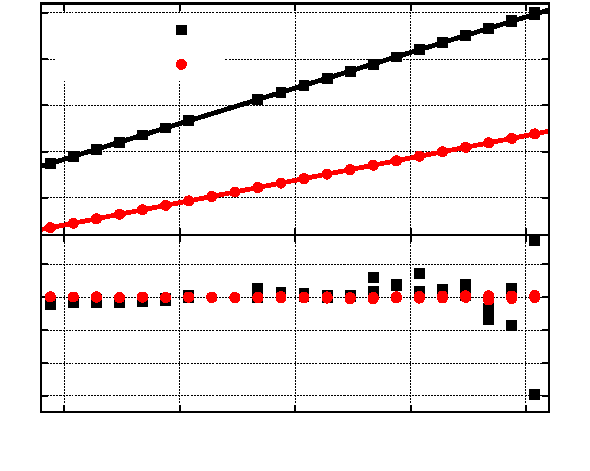
\includegraphics{DistanceCalibrationSAXS}}%
    \gplfronttext
  \end{picture}%
\endgroup
}\label{fig:DistanceCalibrationSAXS}}
		\subfloat[AgBehe at large distance]{\resizebox{0.44\linewidth}{!}{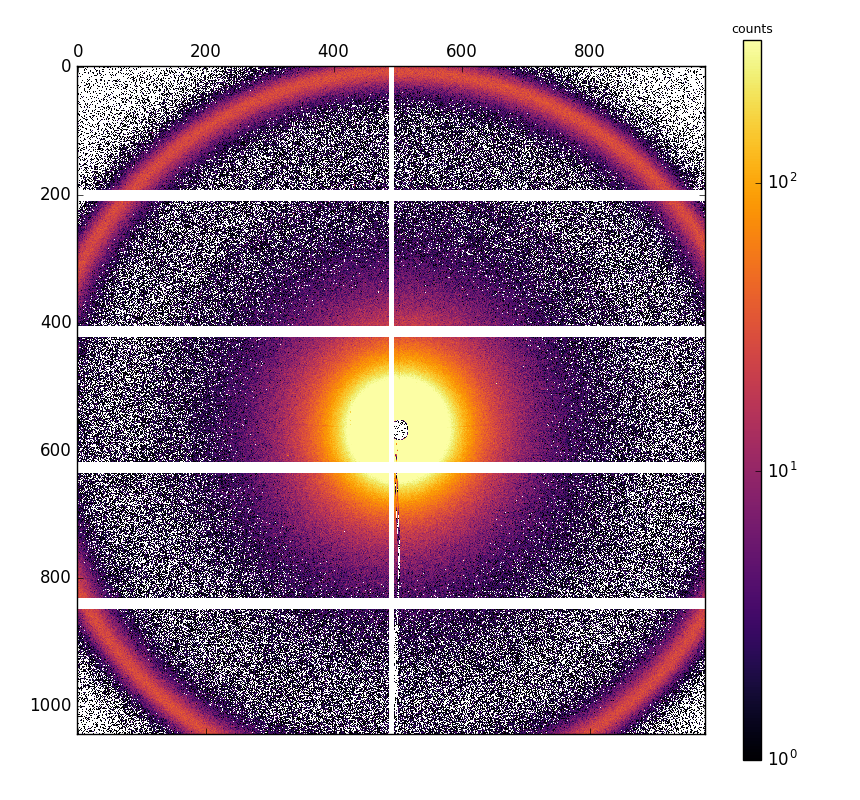
\includegraphics{Figures/AgBeheSAXSLongDistance.png}}\label{fig:AgBeheSAXSLongDistance}}
		\caption{Sample-to-detector distance calibration: a) Radius of the diffraction ring of AgBehe and SBA-15 as a function of the sample-detector distance. A linear function is fitted to obtain the source point distance. The residuals of the fitting are shown in the bottom plot. b) Scattering pattern of AgBehe measured at a distance of 3638.2 mm. The diffraction rings exceeds the detector area. (file "messung kmc daten 2015 1Q pilatus 201501 0394.tif")}
\end{figure}

By measuring the AgBehe pattern along a distance range of 2200 mm with 100 mm steps at 8000 eV, the relative uncertainty associated to the linear fitting is 0.03 $\%$, corresponding to 1.5 mm. As observed in the residuals of the fitting in figure \ref{fig:DistanceCalibrationSAXS}, the deviation increases for long distances, due to the relatively small $d$-spacing of AgBehe, disabling the use of distances larger than $\sim 3600$ mm. In figure \ref{fig:AgBeheSAXSLongDistance}, it is visible how the diffraction ring surpasses the surface of the detector and, thus, diminishes the accuracy of the peak determination.

By using a material with lower $q$-value, such as the templated mesoporous silica SBA-15 \citep{zhao_triblock_1998} ($q=0.681$ nm$^{-1}$), this limitation can be mitigated as shown in figure \ref{fig:DistanceCalibrationSAXS}, where the residuals of SBA are minimal for the entire distance range. By using SBA and increasing the accessible distance range, the relative uncertainty of the fit decreases in a factor 5, reaching an uncertainty of 0.004 $\%$ (0.2 mm) when measuring with 50 mm steps. This improvement is also related with the narrower diffraction peak of SBA-15 (FWHM/$q=2.6\%$) in comparison to AgBehe ($5.5\%$).

Although the fit uncertainty is smaller in the SBA case, the position and shape of diffraction peak depend strongly on the sample preparation (e.g. template pore size). For the same polymer template, the $q$-value of the ring can vary until 1 $\%$ for different thermal treatments and radiation damage effects are visible for short calcination times. On the other side, prolonged beam exposure of AgBehe can damage the sample as well and create small silver nanoparticles, which increase the scattering background \cite{liu_thermal_2006}. The choice of the calibration standard depends strictly on the needs of the experiment. Besides, the largest contributions to the sample-detector distance uncertainty come from the thickness of the sample (ca. 0.5 mm) and from the difference between the calibration with AgBehe and SBA-15 (also 0.5 mm). Normally the uncertainty associated with the distance calibration is $10^{-4}$, similar to the energy resolving power described in section \ref{sec:fcm}.

\section{Sample environment}

The sample consists normally of a few microliters of nanoparticles in solution which are measured in a vacuum-proof container positioned inside the reflectometer. The sample environment must fulfill some requirements:

\begin{itemize}
        \item The container's material should minimize the innecessary absorption of the X-ray photon flux by the sample environment.
        \item The container volume should be small enough to enable the measurement of valuable, limited samples.
        \item The optimal sample thickness for a transmission diffraction experiment is the inverse of its attenuation coefficient $\mu(E)$, which reduces the incoming intensity to $\sim37\%$. For example, the optimal thickness of water at 8000 eV is around 1 mm.
\end{itemize}

Typically, the samples are introduced in thin glass capillaries which maintain the temperature and pressure of the sample close to the ambient conditions. However, there are different sample environments which can be used depending on the requirements of the experiment. In this work, only nanoparticles suspended in aqueous media have been employed, allowing the use of a similar attenuation coefficient for almost all experiments.

\subsection{Round capillaries}

For single-contrast SAXS measurements, borosilicate glass 3.3 round capillaries of 100 mm length were used. They were purchased at WJM Glass (Berlin, Germany) and had a nominal inner diameter of 1 mm and a wall thickness of 10 $\mu$m. The sample is filled into the capillary with a long syringe (Sterican$\textregistered$21 x 4 3/4" , Braun, Melsungen, Germany), avoiding the contact of the needle with the capillary walls. The top end of the capillary is closed by welding.

The very narrow glass walls (with a density of about 2.23 g cm$^{-3}$) absorb only 14 $\%$ of the incoming flux at 8000 eV and produce very low incoherent scattering background. Therefore, these capillaries are suitable for standard SAXS measurements. Unfortunately, the capillaries sample thickness shows a significant deviation along the vertical axis and are inappropriate for measurements at different capillary heights, as needed for the continuous contrast variation technique.

\subsection{Rectangular capillaries}

The capillaries used for the contrast variation experiments are vacuum-proof borosilicate glass capillaries from Hilgenberg (Malsfeld, Germany) with a nominal rectangular cross section of (4.2 $\pm$ 0.2) x (1.25 $\pm$ 0.05) mm$^2$ , a length of (80 $\pm$ 0.5) mm and a wall thickness of ca. 120 $\mu$m. The thicker glass walls reduce the transmitted intensity about $80\%$ at 8000 eV, but in contrast both the glass and sample thicknesses are very homogenous for the entire capillary.

\begin{figure}%[htbp]
	\centering
		\subfloat[Glass thickness]{\resizebox{0.44\linewidth}{!}{% GNUPLOT: LaTeX picture with Postscript
\begingroup
  \makeatletter
  \providecommand\color[2][]{%
    \GenericError{(gnuplot) \space\space\space\@spaces}{%
      Package color not loaded in conjunction with
      terminal option `colourtext'%
    }{See the gnuplot documentation for explanation.%
    }{Either use 'blacktext' in gnuplot or load the package
      color.sty in LaTeX.}%
    \renewcommand\color[2][]{}%
  }%
  \providecommand\includegraphics[2][]{%
    \GenericError{(gnuplot) \space\space\space\@spaces}{%
      Package graphicx or graphics not loaded%
    }{See the gnuplot documentation for explanation.%
    }{The gnuplot epslatex terminal needs graphicx.sty or graphics.sty.}%
    \renewcommand\includegraphics[2][]{}%
  }%
  \providecommand\rotatebox[2]{#2}%
  \@ifundefined{ifGPcolor}{%
    \newif\ifGPcolor
    \GPcolortrue
  }{}%
  \@ifundefined{ifGPblacktext}{%
    \newif\ifGPblacktext
    \GPblacktextfalse
  }{}%
  % define a \g@addto@macro without @ in the name:
  \let\gplgaddtomacro\g@addto@macro
  % define empty templates for all commands taking text:
  \gdef\gplbacktext{}%
  \gdef\gplfronttext{}%
  \makeatother
  \ifGPblacktext
    % no textcolor at all
    \def\colorrgb#1{}%
    \def\colorgray#1{}%
  \else
    % gray or color?
    \ifGPcolor
      \def\colorrgb#1{\color[rgb]{#1}}%
      \def\colorgray#1{\color[gray]{#1}}%
      \expandafter\def\csname LTw\endcsname{\color{white}}%
      \expandafter\def\csname LTb\endcsname{\color{black}}%
      \expandafter\def\csname LTa\endcsname{\color{black}}%
      \expandafter\def\csname LT0\endcsname{\color[rgb]{1,0,0}}%
      \expandafter\def\csname LT1\endcsname{\color[rgb]{0,1,0}}%
      \expandafter\def\csname LT2\endcsname{\color[rgb]{0,0,1}}%
      \expandafter\def\csname LT3\endcsname{\color[rgb]{1,0,1}}%
      \expandafter\def\csname LT4\endcsname{\color[rgb]{0,1,1}}%
      \expandafter\def\csname LT5\endcsname{\color[rgb]{1,1,0}}%
      \expandafter\def\csname LT6\endcsname{\color[rgb]{0,0,0}}%
      \expandafter\def\csname LT7\endcsname{\color[rgb]{1,0.3,0}}%
      \expandafter\def\csname LT8\endcsname{\color[rgb]{0.5,0.5,0.5}}%
    \else
      % gray
      \def\colorrgb#1{\color{black}}%
      \def\colorgray#1{\color[gray]{#1}}%
      \expandafter\def\csname LTw\endcsname{\color{white}}%
      \expandafter\def\csname LTb\endcsname{\color{black}}%
      \expandafter\def\csname LTa\endcsname{\color{black}}%
      \expandafter\def\csname LT0\endcsname{\color{black}}%
      \expandafter\def\csname LT1\endcsname{\color{black}}%
      \expandafter\def\csname LT2\endcsname{\color{black}}%
      \expandafter\def\csname LT3\endcsname{\color{black}}%
      \expandafter\def\csname LT4\endcsname{\color{black}}%
      \expandafter\def\csname LT5\endcsname{\color{black}}%
      \expandafter\def\csname LT6\endcsname{\color{black}}%
      \expandafter\def\csname LT7\endcsname{\color{black}}%
      \expandafter\def\csname LT8\endcsname{\color{black}}%
    \fi
  \fi
  \setlength{\unitlength}{0.0500bp}%
  \begin{picture}(5668.00,4534.00)%
    \gplgaddtomacro\gplbacktext{%
    }%
    \gplgaddtomacro\gplfronttext{%
      \csname LTb\endcsname%
      \put(1241,736){\makebox(0,0){\strut{}-2}}%
      \put(1625,736){\makebox(0,0){\strut{}-1.5}}%
      \put(2009,736){\makebox(0,0){\strut{}-1}}%
      \put(2393,736){\makebox(0,0){\strut{}-0.5}}%
      \put(2777,736){\makebox(0,0){\strut{} 0}}%
      \put(3160,736){\makebox(0,0){\strut{} 0.5}}%
      \put(3544,736){\makebox(0,0){\strut{} 1}}%
      \put(3928,736){\makebox(0,0){\strut{} 1.5}}%
      \put(4312,736){\makebox(0,0){\strut{} 2}}%
      \put(4696,736){\makebox(0,0){\strut{} 2.5}}%
      \put(2834,406){\makebox(0,0){\strut{}Horizontal Position / mm}}%
      \put(801,1022){\makebox(0,0)[r]{\strut{} 5}}%
      \put(801,1304){\makebox(0,0)[r]{\strut{} 5.5}}%
      \put(801,1587){\makebox(0,0)[r]{\strut{} 6}}%
      \put(801,1869){\makebox(0,0)[r]{\strut{} 6.5}}%
      \put(801,2152){\makebox(0,0)[r]{\strut{} 7}}%
      \put(801,2433){\makebox(0,0)[r]{\strut{} 7.5}}%
      \put(801,2715){\makebox(0,0)[r]{\strut{} 8}}%
      \put(801,2998){\makebox(0,0)[r]{\strut{} 8.5}}%
      \put(801,3280){\makebox(0,0)[r]{\strut{} 9}}%
      \put(801,3563){\makebox(0,0)[r]{\strut{} 9.5}}%
      \put(207,2377){\rotatebox{-270}{\makebox(0,0){\strut{}Vertical Position / mm}}}%
      \put(5107,1022){\makebox(0,0)[l]{\strut{}-2}}%
      \put(5107,1473){\makebox(0,0)[l]{\strut{}-1.5}}%
      \put(5107,1925){\makebox(0,0)[l]{\strut{}-1}}%
      \put(5107,2377){\makebox(0,0)[l]{\strut{}-0.5}}%
      \put(5107,2828){\makebox(0,0)[l]{\strut{} 0}}%
      \put(5107,3280){\makebox(0,0)[l]{\strut{} 0.5}}%
      \put(5107,3732){\makebox(0,0)[l]{\strut{} 1}}%
      \put(5701,2377){\rotatebox{270}{\makebox(0,0){\strut{}Deviation /$\%$}}}%
    }%
    \gplbacktext
    \put(0,0){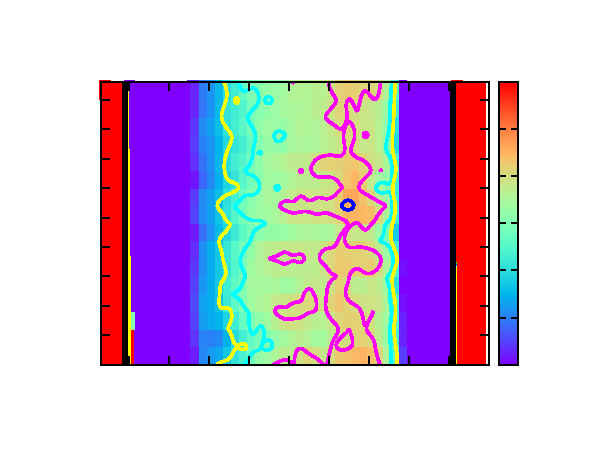
\includegraphics{HilgenbergHomogeneity}}%
    \gplfronttext
  \end{picture}%
\endgroup
}\label{fig:HilgenbergHomogeneity}}
		\subfloat[Sample thickness]{\resizebox{0.44\linewidth}{!}{% GNUPLOT: LaTeX picture with Postscript
\begingroup
  \makeatletter
  \providecommand\color[2][]{%
    \GenericError{(gnuplot) \space\space\space\@spaces}{%
      Package color not loaded in conjunction with
      terminal option `colourtext'%
    }{See the gnuplot documentation for explanation.%
    }{Either use 'blacktext' in gnuplot or load the package
      color.sty in LaTeX.}%
    \renewcommand\color[2][]{}%
  }%
  \providecommand\includegraphics[2][]{%
    \GenericError{(gnuplot) \space\space\space\@spaces}{%
      Package graphicx or graphics not loaded%
    }{See the gnuplot documentation for explanation.%
    }{The gnuplot epslatex terminal needs graphicx.sty or graphics.sty.}%
    \renewcommand\includegraphics[2][]{}%
  }%
  \providecommand\rotatebox[2]{#2}%
  \@ifundefined{ifGPcolor}{%
    \newif\ifGPcolor
    \GPcolortrue
  }{}%
  \@ifundefined{ifGPblacktext}{%
    \newif\ifGPblacktext
    \GPblacktextfalse
  }{}%
  % define a \g@addto@macro without @ in the name:
  \let\gplgaddtomacro\g@addto@macro
  % define empty templates for all commands taking text:
  \gdef\gplbacktext{}%
  \gdef\gplfronttext{}%
  \makeatother
  \ifGPblacktext
    % no textcolor at all
    \def\colorrgb#1{}%
    \def\colorgray#1{}%
  \else
    % gray or color?
    \ifGPcolor
      \def\colorrgb#1{\color[rgb]{#1}}%
      \def\colorgray#1{\color[gray]{#1}}%
      \expandafter\def\csname LTw\endcsname{\color{white}}%
      \expandafter\def\csname LTb\endcsname{\color{black}}%
      \expandafter\def\csname LTa\endcsname{\color{black}}%
      \expandafter\def\csname LT0\endcsname{\color[rgb]{1,0,0}}%
      \expandafter\def\csname LT1\endcsname{\color[rgb]{0,1,0}}%
      \expandafter\def\csname LT2\endcsname{\color[rgb]{0,0,1}}%
      \expandafter\def\csname LT3\endcsname{\color[rgb]{1,0,1}}%
      \expandafter\def\csname LT4\endcsname{\color[rgb]{0,1,1}}%
      \expandafter\def\csname LT5\endcsname{\color[rgb]{1,1,0}}%
      \expandafter\def\csname LT6\endcsname{\color[rgb]{0,0,0}}%
      \expandafter\def\csname LT7\endcsname{\color[rgb]{1,0.3,0}}%
      \expandafter\def\csname LT8\endcsname{\color[rgb]{0.5,0.5,0.5}}%
    \else
      % gray
      \def\colorrgb#1{\color{black}}%
      \def\colorgray#1{\color[gray]{#1}}%
      \expandafter\def\csname LTw\endcsname{\color{white}}%
      \expandafter\def\csname LTb\endcsname{\color{black}}%
      \expandafter\def\csname LTa\endcsname{\color{black}}%
      \expandafter\def\csname LT0\endcsname{\color{black}}%
      \expandafter\def\csname LT1\endcsname{\color{black}}%
      \expandafter\def\csname LT2\endcsname{\color{black}}%
      \expandafter\def\csname LT3\endcsname{\color{black}}%
      \expandafter\def\csname LT4\endcsname{\color{black}}%
      \expandafter\def\csname LT5\endcsname{\color{black}}%
      \expandafter\def\csname LT6\endcsname{\color{black}}%
      \expandafter\def\csname LT7\endcsname{\color{black}}%
      \expandafter\def\csname LT8\endcsname{\color{black}}%
    \fi
  \fi
  \setlength{\unitlength}{0.0500bp}%
  \begin{picture}(5668.00,4534.00)%
    \gplgaddtomacro\gplbacktext{%
    }%
    \gplgaddtomacro\gplfronttext{%
      \csname LTb\endcsname%
      \put(1241,736){\makebox(0,0){\strut{}-2}}%
      \put(2009,736){\makebox(0,0){\strut{}-1}}%
      \put(2777,736){\makebox(0,0){\strut{} 0}}%
      \put(3544,736){\makebox(0,0){\strut{} 1}}%
      \put(4312,736){\makebox(0,0){\strut{} 2}}%
      \put(2834,406){\makebox(0,0){\strut{}Horizontal Position / mm}}%
      \put(801,1323){\makebox(0,0)[r]{\strut{}-4}}%
      \put(801,1926){\makebox(0,0)[r]{\strut{}-2}}%
      \put(801,2527){\makebox(0,0)[r]{\strut{} 0}}%
      \put(801,3130){\makebox(0,0)[r]{\strut{} 2}}%
      \put(801,3732){\makebox(0,0)[r]{\strut{} 4}}%
      \put(471,2377){\rotatebox{-270}{\makebox(0,0){\strut{}Vertical Position / mm}}}%
      \put(5107,1473){\makebox(0,0)[l]{\strut{} 0.99}}%
      \put(5107,2377){\makebox(0,0)[l]{\strut{} 1}}%
      \put(5107,3280){\makebox(0,0)[l]{\strut{} 1.01}}%
      \put(5833,2377){\rotatebox{270}{\makebox(0,0){\strut{}Sample Thickness / mm}}}%
    }%
    \gplbacktext
    \put(0,0){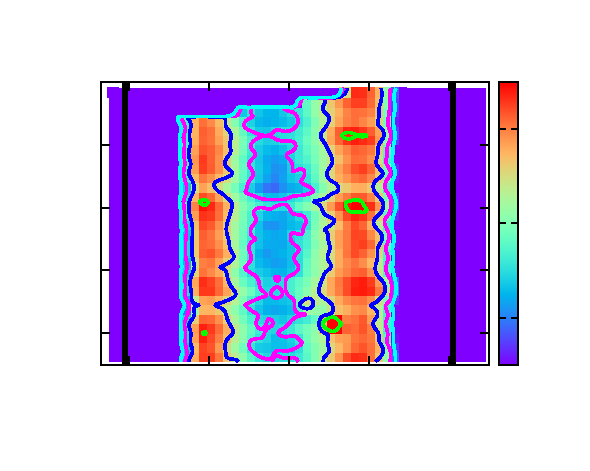
\includegraphics{WaterHomogeneity}}%
    \gplfronttext
  \end{picture}%
\endgroup
}\label{fig:WaterHomogeneity}}
		\caption{Homogeneity of the rectangular capillaries: a) Deviation of the empty capillary tranmission, i.e. glass wall thickness, b) Sample thickness calculated from the water transmission of a filled capillary. }
\end{figure}

The transmission of an empty capillary is mapped in figure \ref{fig:HilgenbergHomogeneity}, where it can be observed that the deviation of the glass wall thickness is less than 2 $\%$ for an horizontal range of 2.5 mm (of a total width of 4.2 mm). This range is at least 5 times larger than the typical beam diameter, avoiding the convolution of different thicknesses in the measurement. Similarly, figure \ref{fig:WaterHomogeneity} depicts the sample thickness in the capillary, calculated from a capillary filled with water using the Beer-Lambert law, the glass transmission and the mass attenuation coefficient of water at 8000 eV, 10.37 cm$^{2}$ g$^{-1}$ \citep{hubbell_tables_1996}. The thickness of the sample introduced in the capillary is homogenous within 2 $\%$ for a width range of ca. 2.5 mm. 

\begin{figure}%[htbp]
	\centering
		% GNUPLOT: LaTeX picture with Postscript
\begingroup
  \makeatletter
  \providecommand\color[2][]{%
    \GenericError{(gnuplot) \space\space\space\@spaces}{%
      Package color not loaded in conjunction with
      terminal option `colourtext'%
    }{See the gnuplot documentation for explanation.%
    }{Either use 'blacktext' in gnuplot or load the package
      color.sty in LaTeX.}%
    \renewcommand\color[2][]{}%
  }%
  \providecommand\includegraphics[2][]{%
    \GenericError{(gnuplot) \space\space\space\@spaces}{%
      Package graphicx or graphics not loaded%
    }{See the gnuplot documentation for explanation.%
    }{The gnuplot epslatex terminal needs graphicx.sty or graphics.sty.}%
    \renewcommand\includegraphics[2][]{}%
  }%
  \providecommand\rotatebox[2]{#2}%
  \@ifundefined{ifGPcolor}{%
    \newif\ifGPcolor
    \GPcolortrue
  }{}%
  \@ifundefined{ifGPblacktext}{%
    \newif\ifGPblacktext
    \GPblacktextfalse
  }{}%
  % define a \g@addto@macro without @ in the name:
  \let\gplgaddtomacro\g@addto@macro
  % define empty templates for all commands taking text:
  \gdef\gplbacktext{}%
  \gdef\gplfronttext{}%
  \makeatother
  \ifGPblacktext
    % no textcolor at all
    \def\colorrgb#1{}%
    \def\colorgray#1{}%
  \else
    % gray or color?
    \ifGPcolor
      \def\colorrgb#1{\color[rgb]{#1}}%
      \def\colorgray#1{\color[gray]{#1}}%
      \expandafter\def\csname LTw\endcsname{\color{white}}%
      \expandafter\def\csname LTb\endcsname{\color{black}}%
      \expandafter\def\csname LTa\endcsname{\color{black}}%
      \expandafter\def\csname LT0\endcsname{\color[rgb]{1,0,0}}%
      \expandafter\def\csname LT1\endcsname{\color[rgb]{0,1,0}}%
      \expandafter\def\csname LT2\endcsname{\color[rgb]{0,0,1}}%
      \expandafter\def\csname LT3\endcsname{\color[rgb]{1,0,1}}%
      \expandafter\def\csname LT4\endcsname{\color[rgb]{0,1,1}}%
      \expandafter\def\csname LT5\endcsname{\color[rgb]{1,1,0}}%
      \expandafter\def\csname LT6\endcsname{\color[rgb]{0,0,0}}%
      \expandafter\def\csname LT7\endcsname{\color[rgb]{1,0.3,0}}%
      \expandafter\def\csname LT8\endcsname{\color[rgb]{0.5,0.5,0.5}}%
    \else
      % gray
      \def\colorrgb#1{\color{black}}%
      \def\colorgray#1{\color[gray]{#1}}%
      \expandafter\def\csname LTw\endcsname{\color{white}}%
      \expandafter\def\csname LTb\endcsname{\color{black}}%
      \expandafter\def\csname LTa\endcsname{\color{black}}%
      \expandafter\def\csname LT0\endcsname{\color{black}}%
      \expandafter\def\csname LT1\endcsname{\color{black}}%
      \expandafter\def\csname LT2\endcsname{\color{black}}%
      \expandafter\def\csname LT3\endcsname{\color{black}}%
      \expandafter\def\csname LT4\endcsname{\color{black}}%
      \expandafter\def\csname LT5\endcsname{\color{black}}%
      \expandafter\def\csname LT6\endcsname{\color{black}}%
      \expandafter\def\csname LT7\endcsname{\color{black}}%
      \expandafter\def\csname LT8\endcsname{\color{black}}%
    \fi
  \fi
  \setlength{\unitlength}{0.0500bp}%
  \begin{picture}(5668.00,4534.00)%
    \gplgaddtomacro\gplbacktext{%
      \csname LTb\endcsname%
      \put(858,921){\makebox(0,0)[r]{\strut{} 0.07}}%
      \put(858,1964){\makebox(0,0)[r]{\strut{} 0.1}}%
      \put(858,3149){\makebox(0,0)[r]{\strut{} 0.15}}%
      \put(858,3990){\makebox(0,0)[r]{\strut{} 0.2}}%
      \put(1275,484){\makebox(0,0){\strut{}-4}}%
      \put(1846,484){\makebox(0,0){\strut{}-2}}%
      \put(2417,484){\makebox(0,0){\strut{} 0}}%
      \put(2988,484){\makebox(0,0){\strut{} 2}}%
      \put(3559,484){\makebox(0,0){\strut{} 4}}%
      \put(4129,484){\makebox(0,0){\strut{} 6}}%
      \put(4700,484){\makebox(0,0){\strut{} 8}}%
      \put(5271,484){\makebox(0,0){\strut{} 10}}%
      \put(220,2486){\rotatebox{-270}{\makebox(0,0){\strut{}Transmission}}}%
      \put(3130,154){\makebox(0,0){\strut{}Vertical position / mm}}%
    }%
    \gplgaddtomacro\gplfronttext{%
      \csname LTb\endcsname%
      \put(2475,3730){\makebox(0,0)[r]{\strut{}Transmission}}%
      \csname LTb\endcsname%
      \put(2475,3510){\makebox(0,0)[r]{\strut{}Glass only}}%
      \csname LTb\endcsname%
      \put(2475,3290){\makebox(0,0)[r]{\strut{}H$_2$O}}%
    }%
    \gplbacktext
    \put(0,0){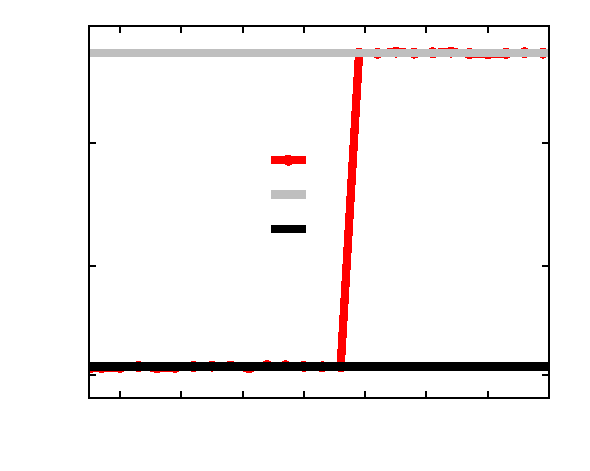
\includegraphics{GaldenCalibration}}%
    \gplfronttext
  \end{picture}%
\endgroup

		\caption{X-ray transmission of a rectangular capillary half-filled with water along the main vertical axis situated at $x=-0.15$ mm.}
		\label{fig:GaldenCalibration}
\end{figure}

From these figures, it is clear that the homogeneity of the sample environment is even better along the main vertical axis of the capillary. Figure \ref{fig:GaldenCalibration} shows the measured X-ray transmission of a half-filled capillary along its vertical axis (at the horizontal position -0.15 mm). For example, the glass transmission within a 6 mm vertical range is $20.1\%$, with an associated relative uncertainty of $\delta_r T =0.6 \; \%$. By calculating $\delta_r d = \frac{\delta_r T}{log(T)}$ where $T$ is the glass transmission, the relative uncertainty of the glass thickness is $\delta_r d = 0.4 \; \%$. Analogously, the uncertainty of the water transmission is 0.9 $\%$ and the sample thicknes has an uncertainty of 0.9 $\%$ along the vertical axis.

These rectangular capillaries are a very suitable sample environment for measurements which require a high homogeneity along the vertical axis of the capillary. The thickness of the wall varies only 0.4 $\%$ and the sample thickness less than 0.9 $\%$, although the thick glass walls reduce considerably the transmitted intensity and produce larger background scattering than the round capillaries.

\subsection{Cell for low-energies}

Samples with larger structures require the measurement of scattering curves at lower $q$-values. To extend the measurable $q$-range, one possibility is to reduce the photon beam energy, though this involves reducing the sample thickness, due to the short penetration length of X-rays at low energies. Therefore, a custom-made sample holder is used utilizing silicon-nitride windows (NX7150E, Norcada Inc., Edmonton,Canada). The 500 nm thickness windows produce very low scattering and have a negligable absorbance ($<5\;\%$) for energies above 4000 eV.

A polymeric 100 $\mu$m ring cut with a microtome is used as spacer between the 2 windows, in order to achieve the desired 120 $\mu$m sample thickness which optimizes the intensity attenuation at 4000 eV. The acces to smaller $q$-values using this cell is shown in \cite{varga_towards_2014}, where a value of $q=0.015$ nm$^{-1}$ is achieved.

\begin{figure}%[htbp]
	\centering
		\resizebox{0.7\linewidth}{!}{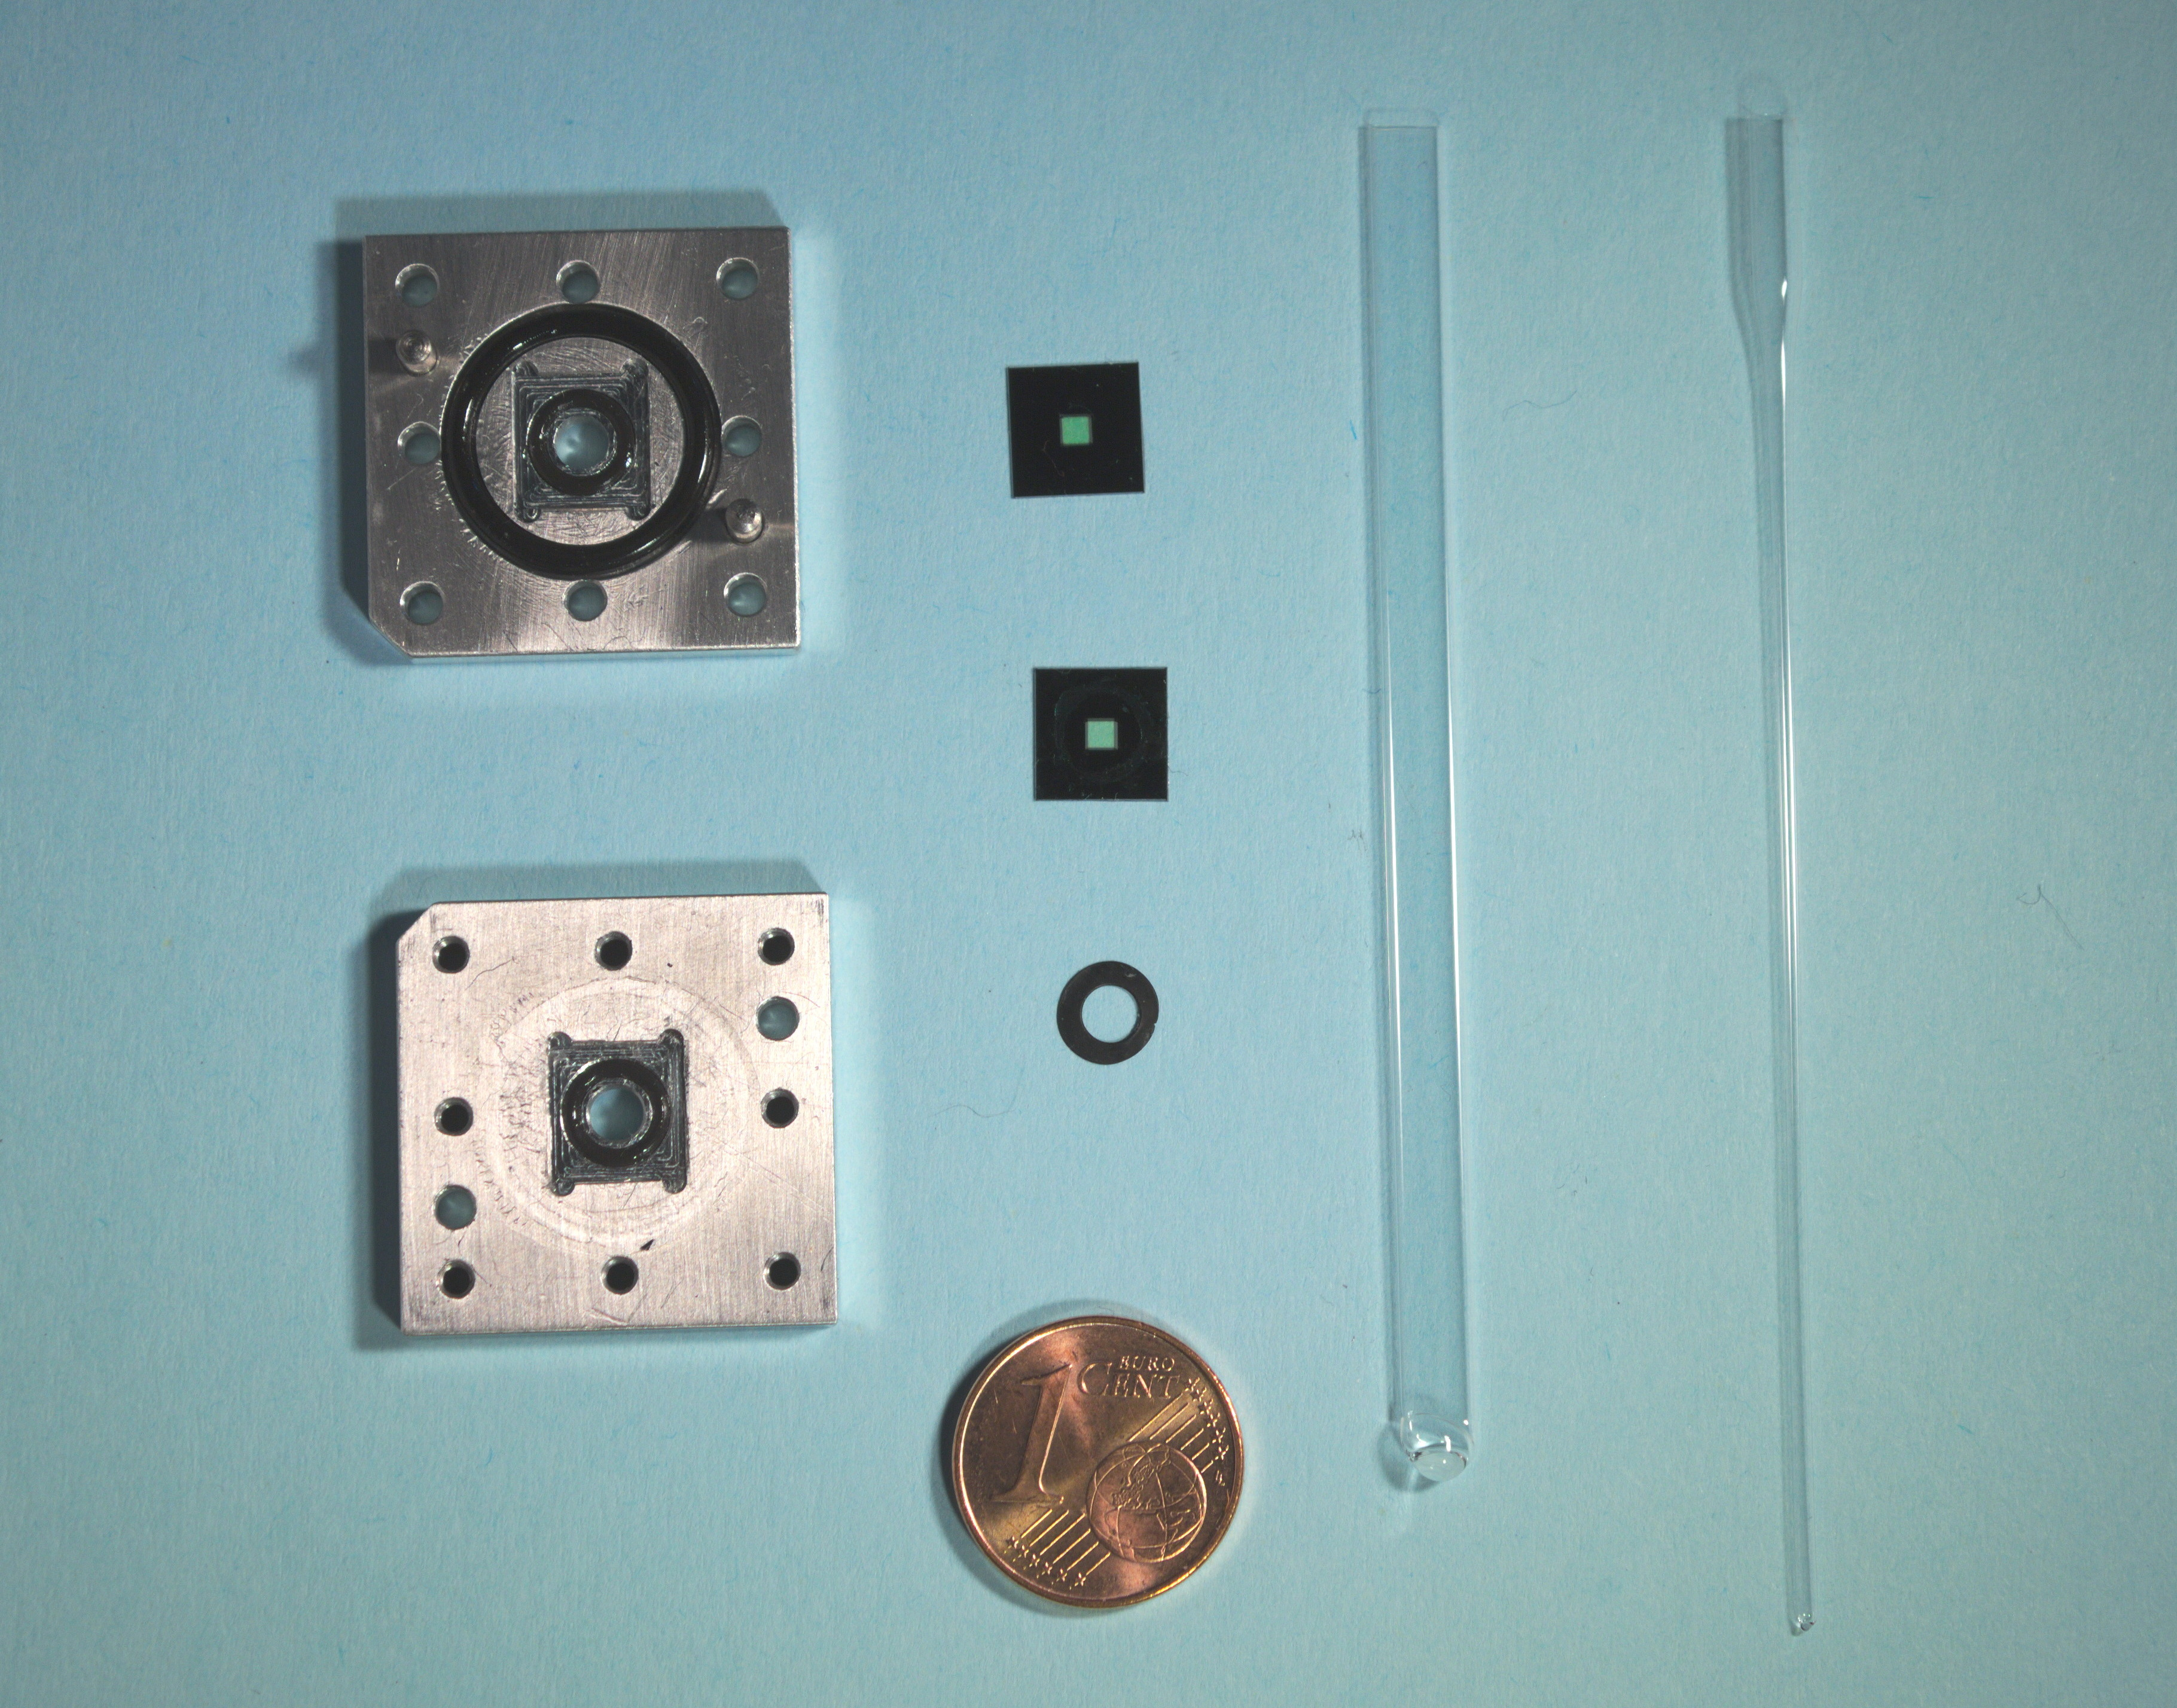
\includegraphics{Figures/SampleEnvironment.jpg}}
		\caption{Different sample environments: Round and rectangular capillaries and disassembled cell with the two silicon-nitride windows, the polymeric spacer and the metallic holder.}
		\label{fig:SampleEnvironment}
\end{figure}

\section{Obtention of the scattering curves}

The obtained scattering curve was normalized to the exposure time, the measured suspension transmittance and the incident photon flux, measured by means of a calibrated transparent silicon diode. 

Radial integration and error propagation

\subsection{Absolute intensity calibration}

lupolen as standard material \cite{kratky_absolute_1966,shaffer_calibration_1974}

glassy carbon \cite{perret_glassy_1972}

use the knowledge from the innanopart project??????
\subsubsection{Flux monitor}
thin diode
\subsubsection{Detector efficiceny}
pilatus and thin diode





















\textcolor{red}{-----------------------THIS SHOULD ALL GO TO THE NEXT CHAPTER-----------------------}











\section{Small-angle X-ray scattering: DIRECT FROM PAPER}
The measurements were performed at the four-crystal monochromator beamline in the PTB laboratory at the electron storage ring BESSY II (Berlin, \emph{Germany}), which provides highly intense, collimated synchrotron radiation focused on the sample and collimated into a \(0.5\) mm circular spot by Ge pinholes situated between the sample and the monochromator with an energy resolving power \( E/\Delta E \) of \( 10^4 \). To measure the total flux and sample transmission, photodiodes were used which were calibrated against a cryogenic electric substitution radiometer with a relative uncertainty of \( 1\,\% \) \cite{krumrey_high-accuracy_2001}.


\begin{figure}%[htbp]
	\centering
		\input{Figures/DensityGradientCapillarySetup.pdf_tex}
		\caption{The rectangular density gradient capillary is placed in the X-ray beam and can be moved by sample motors in both directions perpendicular to the incoming beam.}
		\label{fig:DensityGradientCapillarySetup}
\end{figure}

The rectangular capillary is placed in a sample holder which allows the movement with micrometer precision in the directions perpendicular to the incoming beam, as depicted in figure \ref{fig:DensityGradientCapillarySetup}. In order to determine the central vertical capillary axis, a horizontal X-ray transmission scan is performed at two different vertical positions of the capillary spaced by 20 mm. The central vertical axis can be drawn from the centers of both measurements and the sample can be moved along this axis by the simultaneous operation of the vertical and horizontal motors.

The sample was moved in steps of 0.5 mm along the central vertical capillary axis and exposed at each position for 45 seconds. At these positions, the solution transmittances were previously measured and the suspending medium electron density calibrated. The measured scattering curve is an average over a range of solvent electron densities associated with the beam size. The momentum transfer \(q\) of the scattering curves was calculated using
\begin{equation}
q=\frac{4\pi E}{hc}\sin\theta ,
\end{equation}
where \(\theta\) is half of the scattering angle, \(h\) is the Planck constant and \(c\) is the speed of light. The incident photon energy \(E = \left(8800.0  \pm 0.8\right)\) eV was chosen to be higher than the photon energy for the transmission measurements to improve the recorded statistics, due to a ca. \(150\) higher transmission \cite{henke_x-ray_1993}. The scattered X-ray photons were collected with a vacuum-compatible Pilatus 1M hybrid-pixel detector (Dectris Ltd, (Baden, \emph{Switzerland})) with a pixel size of \(d = \left(172.1  \pm 0.2\right) \; \mu \)m at a distance \(L = \left(4540.2  \pm 0.8\right)\) mm from the capillaries, determined by triangulation using a calibrated length measurement system \cite{wernecke_characterization_2014}. The obtained scattering curve was normalized to the exposure time and the incident intensity, measured by means of a calibrated transparent silicon diode.  In total, 40 scattering curves with different solvent electron densities were measured at two different times \(t_1=\)78 min and \(t_2=\)156 min after filling the capillaries.


\subsection{Filling of capilaries}
galden at bottom, reference layer


\subsection{Calibration of solvent density and finding of main axis}
The transmitted intensity through the sample is recorded at a photon energy of \(E = (5500.0 \pm  0.5)\) eV for 10 seconds at each position. The measurement consists of 20 points spaced 0.5 mm along the central vertical axis of the capillary. The overall X-ray transmission measurement requires approximately 5 minutes, which is within the calculated diffusion timescale of the aqueous sucrose solution. The solvent electron density profile within the density gradient capillary derived from this measurement is depicted in figure \textcolor{red}{NO IMAGE CORRESPONDING TO THIS MEASUREMENT HAS BEEN ADDED}. A uniform thickness of the capillary within $0.5\,\%$ along this axis was determined by measuring the X-ray transmission of an empty capillary. The associated uncertainty in the sample transmission measurement is below $4\,\%$. The sample thickness is assumed to be constant. This transmission measurement is performed both immediately before and after recording the scattering patterns, which takes 15 minutes to complete. The transmittance values used for the density calibration are then linearly interpolated between both data sets taking into account the time-dependence. These values can be converted to solvent electron densities via the Beer-Lambert law, which relates the density of the solution with the transmitted intensity:
\begin{equation}
  \rho(z) = A \left( \ln{I_0} - \ln{I(z)} \right) .
\end{equation}
Here \(\rho\) is the electron density of the suspending medium, $I$ and $I_0$ are the transmitted and incoming intensities respectively and $A$ is a factor determined by the reference values of the solvent electron density at the vertical limits of the capillary at the initial time. The sucrose concentration in solution expressed as the mass fraction \( M \) at these reference points can be converted to electron densities with the empirical formula \( \rho=1.2681M+333.19 \) nm\(^{-3}\) \citep{haynes_crc_2012}. The suspending medium electron density shows a maximum uncertainty of 1 nm$^{-3}$ associated with the vertical size of the focused X-ray beam.

X-ray transmission measurements at the aqueous sucrose gradient were performed at a lower incident photon energy $E = 5500$ eV to increase the transmittance differences for the less absorbing sucrose solution by a factor of 5.

\begin{figure}%[htbp]
	\centering
		% GNUPLOT: LaTeX picture with Postscript
\begingroup
  \makeatletter
  \providecommand\color[2][]{%
    \GenericError{(gnuplot) \space\space\space\@spaces}{%
      Package color not loaded in conjunction with
      terminal option `colourtext'%
    }{See the gnuplot documentation for explanation.%
    }{Either use 'blacktext' in gnuplot or load the package
      color.sty in LaTeX.}%
    \renewcommand\color[2][]{}%
  }%
  \providecommand\includegraphics[2][]{%
    \GenericError{(gnuplot) \space\space\space\@spaces}{%
      Package graphicx or graphics not loaded%
    }{See the gnuplot documentation for explanation.%
    }{The gnuplot epslatex terminal needs graphicx.sty or graphics.sty.}%
    \renewcommand\includegraphics[2][]{}%
  }%
  \providecommand\rotatebox[2]{#2}%
  \@ifundefined{ifGPcolor}{%
    \newif\ifGPcolor
    \GPcolortrue
  }{}%
  \@ifundefined{ifGPblacktext}{%
    \newif\ifGPblacktext
    \GPblacktextfalse
  }{}%
  % define a \g@addto@macro without @ in the name:
  \let\gplgaddtomacro\g@addto@macro
  % define empty templates for all commands taking text:
  \gdef\gplbacktext{}%
  \gdef\gplfronttext{}%
  \makeatother
  \ifGPblacktext
    % no textcolor at all
    \def\colorrgb#1{}%
    \def\colorgray#1{}%
  \else
    % gray or color?
    \ifGPcolor
      \def\colorrgb#1{\color[rgb]{#1}}%
      \def\colorgray#1{\color[gray]{#1}}%
      \expandafter\def\csname LTw\endcsname{\color{white}}%
      \expandafter\def\csname LTb\endcsname{\color{black}}%
      \expandafter\def\csname LTa\endcsname{\color{black}}%
      \expandafter\def\csname LT0\endcsname{\color[rgb]{1,0,0}}%
      \expandafter\def\csname LT1\endcsname{\color[rgb]{0,1,0}}%
      \expandafter\def\csname LT2\endcsname{\color[rgb]{0,0,1}}%
      \expandafter\def\csname LT3\endcsname{\color[rgb]{1,0,1}}%
      \expandafter\def\csname LT4\endcsname{\color[rgb]{0,1,1}}%
      \expandafter\def\csname LT5\endcsname{\color[rgb]{1,1,0}}%
      \expandafter\def\csname LT6\endcsname{\color[rgb]{0,0,0}}%
      \expandafter\def\csname LT7\endcsname{\color[rgb]{1,0.3,0}}%
      \expandafter\def\csname LT8\endcsname{\color[rgb]{0.5,0.5,0.5}}%
    \else
      % gray
      \def\colorrgb#1{\color{black}}%
      \def\colorgray#1{\color[gray]{#1}}%
      \expandafter\def\csname LTw\endcsname{\color{white}}%
      \expandafter\def\csname LTb\endcsname{\color{black}}%
      \expandafter\def\csname LTa\endcsname{\color{black}}%
      \expandafter\def\csname LT0\endcsname{\color{black}}%
      \expandafter\def\csname LT1\endcsname{\color{black}}%
      \expandafter\def\csname LT2\endcsname{\color{black}}%
      \expandafter\def\csname LT3\endcsname{\color{black}}%
      \expandafter\def\csname LT4\endcsname{\color{black}}%
      \expandafter\def\csname LT5\endcsname{\color{black}}%
      \expandafter\def\csname LT6\endcsname{\color{black}}%
      \expandafter\def\csname LT7\endcsname{\color{black}}%
      \expandafter\def\csname LT8\endcsname{\color{black}}%
    \fi
  \fi
    \setlength{\unitlength}{0.0500bp}%
    \ifx\gptboxheight\undefined%
      \newlength{\gptboxheight}%
      \newlength{\gptboxwidth}%
      \newsavebox{\gptboxtext}%
    \fi%
    \setlength{\fboxrule}{0.5pt}%
    \setlength{\fboxsep}{1pt}%
\begin{picture}(8502.00,4534.00)%
    \gplgaddtomacro\gplbacktext{%
      \csname LTb\endcsname%
      \put(550,815){\makebox(0,0)[r]{\strut{}$0$}}%
      \csname LTb\endcsname%
      \put(550,1239){\makebox(0,0)[r]{\strut{}$5$}}%
      \csname LTb\endcsname%
      \put(550,1663){\makebox(0,0)[r]{\strut{}$10$}}%
      \csname LTb\endcsname%
      \put(550,2087){\makebox(0,0)[r]{\strut{}$15$}}%
      \csname LTb\endcsname%
      \put(550,2511){\makebox(0,0)[r]{\strut{}$20$}}%
      \csname LTb\endcsname%
      \put(550,2935){\makebox(0,0)[r]{\strut{}$25$}}%
      \csname LTb\endcsname%
      \put(550,3359){\makebox(0,0)[r]{\strut{}$30$}}%
      \csname LTb\endcsname%
      \put(550,3783){\makebox(0,0)[r]{\strut{}$35$}}%
      \csname LTb\endcsname%
      \put(550,4206){\makebox(0,0)[r]{\strut{}$40$}}%
      \csname LTb\endcsname%
      \put(682,484){\makebox(0,0){\strut{}$0$}}%
      \csname LTb\endcsname%
      \put(1456,484){\makebox(0,0){\strut{}$2$}}%
      \csname LTb\endcsname%
      \put(2230,484){\makebox(0,0){\strut{}$4$}}%
      \csname LTb\endcsname%
      \put(3004,484){\makebox(0,0){\strut{}$6$}}%
      \csname LTb\endcsname%
      \put(3778,484){\makebox(0,0){\strut{}$8$}}%
      \csname LTb\endcsname%
      \put(4552,484){\makebox(0,0){\strut{}$10$}}%
      \csname LTb\endcsname%
      \put(5326,484){\makebox(0,0){\strut{}$12$}}%
      \csname LTb\endcsname%
      \put(6100,484){\makebox(0,0){\strut{}$14$}}%
      \put(6425,4187){\makebox(0,0)[l]{\strut{}$1.2$}}%
      \put(6425,3202){\makebox(0,0)[l]{\strut{}$2$}}%
      \put(6425,1864){\makebox(0,0)[l]{\strut{}$4$}}%
      \put(6425,785){\makebox(0,0)[l]{\strut{}$7$}}%
    }%
    \gplgaddtomacro\gplfronttext{%
      \csname LTb\endcsname%
      \put(176,2486){\rotatebox{-270}{\makebox(0,0){\strut{}Particle Mass Concentration / $\%$}}}%
      \put(6732,2486){\rotatebox{270}{\makebox(0,0){\strut{}X-ray Transmission / $\%$}}}%
      \put(3487,154){\makebox(0,0){\strut{}Vertical Position / mm}}%
      \csname LTb\endcsname%
      \put(7505,704){\makebox(0,0)[l]{\strut{}\smaller 100}}%
      \put(7505,1213){\makebox(0,0)[l]{\strut{}\smaller 120}}%
      \put(7505,1722){\makebox(0,0)[l]{\strut{}\smaller 140}}%
      \put(7505,2231){\makebox(0,0)[l]{\strut{}\smaller 160}}%
      \put(7505,2741){\makebox(0,0)[l]{\strut{}\smaller 180}}%
      \put(7505,3250){\makebox(0,0)[l]{\strut{}\smaller 200}}%
      \put(7505,3759){\makebox(0,0)[l]{\strut{}\smaller 220}}%
      \put(7505,4269){\makebox(0,0)[l]{\strut{}\smaller 240}}%
      \put(7968,2486){\rotatebox{270}{\makebox(0,0){\strut{}\smaller Diffusion Time / min}}}%
    }%
    \gplbacktext
    \put(0,0){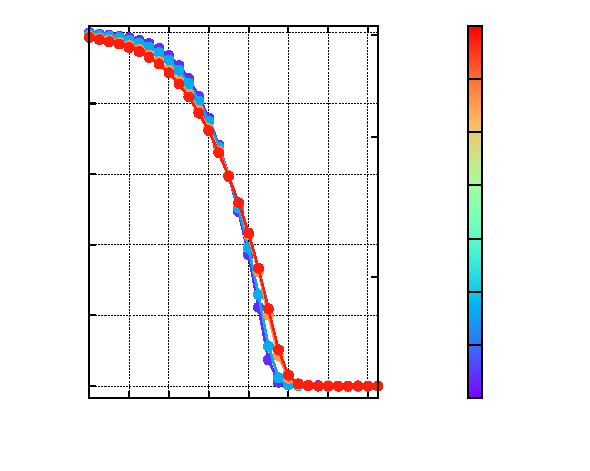
\includegraphics{LudoxHS40TransmissionCalibration}}%
    \gplfronttext
  \end{picture}%
\endgroup

		\caption{Typical measurement of particles with different diffusion timescale: Sucrose (with Kisker NPs) measured at 5500 eV and Colloids (Ludox HS40) mesaured at 8000eV}
		\label{fig:LudoxHS40TransmissionCalibration}
\end{figure}

\begin{figure}%[htbp]
	\centering
		% GNUPLOT: LaTeX picture with Postscript
\begingroup
  \makeatletter
  \providecommand\color[2][]{%
    \GenericError{(gnuplot) \space\space\space\@spaces}{%
      Package color not loaded in conjunction with
      terminal option `colourtext'%
    }{See the gnuplot documentation for explanation.%
    }{Either use 'blacktext' in gnuplot or load the package
      color.sty in LaTeX.}%
    \renewcommand\color[2][]{}%
  }%
  \providecommand\includegraphics[2][]{%
    \GenericError{(gnuplot) \space\space\space\@spaces}{%
      Package graphicx or graphics not loaded%
    }{See the gnuplot documentation for explanation.%
    }{The gnuplot epslatex terminal needs graphicx.sty or graphics.sty.}%
    \renewcommand\includegraphics[2][]{}%
  }%
  \providecommand\rotatebox[2]{#2}%
  \@ifundefined{ifGPcolor}{%
    \newif\ifGPcolor
    \GPcolortrue
  }{}%
  \@ifundefined{ifGPblacktext}{%
    \newif\ifGPblacktext
    \GPblacktextfalse
  }{}%
  % define a \g@addto@macro without @ in the name:
  \let\gplgaddtomacro\g@addto@macro
  % define empty templates for all commands taking text:
  \gdef\gplbacktext{}%
  \gdef\gplfronttext{}%
  \makeatother
  \ifGPblacktext
    % no textcolor at all
    \def\colorrgb#1{}%
    \def\colorgray#1{}%
  \else
    % gray or color?
    \ifGPcolor
      \def\colorrgb#1{\color[rgb]{#1}}%
      \def\colorgray#1{\color[gray]{#1}}%
      \expandafter\def\csname LTw\endcsname{\color{white}}%
      \expandafter\def\csname LTb\endcsname{\color{black}}%
      \expandafter\def\csname LTa\endcsname{\color{black}}%
      \expandafter\def\csname LT0\endcsname{\color[rgb]{1,0,0}}%
      \expandafter\def\csname LT1\endcsname{\color[rgb]{0,1,0}}%
      \expandafter\def\csname LT2\endcsname{\color[rgb]{0,0,1}}%
      \expandafter\def\csname LT3\endcsname{\color[rgb]{1,0,1}}%
      \expandafter\def\csname LT4\endcsname{\color[rgb]{0,1,1}}%
      \expandafter\def\csname LT5\endcsname{\color[rgb]{1,1,0}}%
      \expandafter\def\csname LT6\endcsname{\color[rgb]{0,0,0}}%
      \expandafter\def\csname LT7\endcsname{\color[rgb]{1,0.3,0}}%
      \expandafter\def\csname LT8\endcsname{\color[rgb]{0.5,0.5,0.5}}%
    \else
      % gray
      \def\colorrgb#1{\color{black}}%
      \def\colorgray#1{\color[gray]{#1}}%
      \expandafter\def\csname LTw\endcsname{\color{white}}%
      \expandafter\def\csname LTb\endcsname{\color{black}}%
      \expandafter\def\csname LTa\endcsname{\color{black}}%
      \expandafter\def\csname LT0\endcsname{\color{black}}%
      \expandafter\def\csname LT1\endcsname{\color{black}}%
      \expandafter\def\csname LT2\endcsname{\color{black}}%
      \expandafter\def\csname LT3\endcsname{\color{black}}%
      \expandafter\def\csname LT4\endcsname{\color{black}}%
      \expandafter\def\csname LT5\endcsname{\color{black}}%
      \expandafter\def\csname LT6\endcsname{\color{black}}%
      \expandafter\def\csname LT7\endcsname{\color{black}}%
      \expandafter\def\csname LT8\endcsname{\color{black}}%
    \fi
  \fi
    \setlength{\unitlength}{0.0500bp}%
    \ifx\gptboxheight\undefined%
      \newlength{\gptboxheight}%
      \newlength{\gptboxwidth}%
      \newsavebox{\gptboxtext}%
    \fi%
    \setlength{\fboxrule}{0.5pt}%
    \setlength{\fboxsep}{1pt}%
\begin{picture}(8502.00,4534.00)%
    \gplgaddtomacro\gplbacktext{%
      \csname LTb\endcsname%
      \put(594,1050){\makebox(0,0)[r]{\strut{}$335$}}%
      \csname LTb\endcsname%
      \put(594,1614){\makebox(0,0)[r]{\strut{}$340$}}%
      \csname LTb\endcsname%
      \put(594,2178){\makebox(0,0)[r]{\strut{}$345$}}%
      \csname LTb\endcsname%
      \put(594,2742){\makebox(0,0)[r]{\strut{}$350$}}%
      \csname LTb\endcsname%
      \put(594,3306){\makebox(0,0)[r]{\strut{}$355$}}%
      \csname LTb\endcsname%
      \put(594,3870){\makebox(0,0)[r]{\strut{}$360$}}%
      \csname LTb\endcsname%
      \put(951,484){\makebox(0,0){\strut{}$0$}}%
      \csname LTb\endcsname%
      \put(1851,484){\makebox(0,0){\strut{}$2$}}%
      \csname LTb\endcsname%
      \put(2751,484){\makebox(0,0){\strut{}$4$}}%
      \csname LTb\endcsname%
      \put(3651,484){\makebox(0,0){\strut{}$6$}}%
      \csname LTb\endcsname%
      \put(4551,484){\makebox(0,0){\strut{}$8$}}%
      \csname LTb\endcsname%
      \put(5451,484){\makebox(0,0){\strut{}$10$}}%
      \put(6033,3996){\makebox(0,0)[l]{\strut{}$0.027$}}%
      \put(6033,3109){\makebox(0,0)[l]{\strut{}$0.028$}}%
      \put(6033,1835){\makebox(0,0)[l]{\strut{}$0.0295$}}%
      \put(6033,1022){\makebox(0,0)[l]{\strut{}$0.0305$}}%
    }%
    \gplgaddtomacro\gplfronttext{%
      \csname LTb\endcsname%
      \put(220,2486){\rotatebox{-270}{\makebox(0,0){\strut{}Solvent electron density / nm$^{-3}$}}}%
      \put(6736,2486){\rotatebox{270}{\makebox(0,0){\strut{}X-ray Transmission / $\%$}}}%
      \put(3313,154){\makebox(0,0){\strut{}Vertical Position / mm}}%
      \csname LTb\endcsname%
      \put(7476,704){\makebox(0,0)[l]{\strut{}\smaller 100}}%
      \put(7476,1213){\makebox(0,0)[l]{\strut{}\smaller 120}}%
      \put(7476,1722){\makebox(0,0)[l]{\strut{}\smaller 140}}%
      \put(7476,2231){\makebox(0,0)[l]{\strut{}\smaller 160}}%
      \put(7476,2741){\makebox(0,0)[l]{\strut{}\smaller 180}}%
      \put(7476,3250){\makebox(0,0)[l]{\strut{}\smaller 200}}%
      \put(7476,3759){\makebox(0,0)[l]{\strut{}\smaller 220}}%
      \put(7476,4269){\makebox(0,0)[l]{\strut{}\smaller 240}}%
      \put(7939,2486){\rotatebox{270}{\makebox(0,0){\strut{}\smaller Diffusion Time / min}}}%
    }%
    \gplbacktext
    \put(0,0){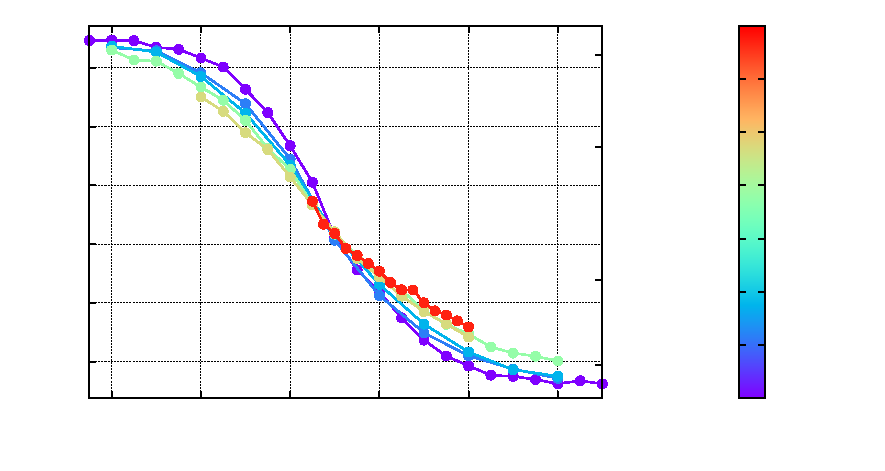
\includegraphics{KiskerTransmissionCalibration}}%
    \gplfronttext
  \end{picture}%
\endgroup

		\caption{Typical measurement of particles with different diffusion timescale: Sucrose (with Kisker NPs) measured at 5500 eV and Colloids (Ludox HS40) mesaured at 8000eV}
		\label{fig:KiskerTransmissionCalibration}
\end{figure}

\begin{figure}%[htbp]
	\centering
		\subfloat[Transmission calculation]{\resizebox{0.44\linewidth}{!}{% GNUPLOT: LaTeX picture with Postscript
\begingroup
  \makeatletter
  \providecommand\color[2][]{%
    \GenericError{(gnuplot) \space\space\space\@spaces}{%
      Package color not loaded in conjunction with
      terminal option `colourtext'%
    }{See the gnuplot documentation for explanation.%
    }{Either use 'blacktext' in gnuplot or load the package
      color.sty in LaTeX.}%
    \renewcommand\color[2][]{}%
  }%
  \providecommand\includegraphics[2][]{%
    \GenericError{(gnuplot) \space\space\space\@spaces}{%
      Package graphicx or graphics not loaded%
    }{See the gnuplot documentation for explanation.%
    }{The gnuplot epslatex terminal needs graphicx.sty or graphics.sty.}%
    \renewcommand\includegraphics[2][]{}%
  }%
  \providecommand\rotatebox[2]{#2}%
  \@ifundefined{ifGPcolor}{%
    \newif\ifGPcolor
    \GPcolortrue
  }{}%
  \@ifundefined{ifGPblacktext}{%
    \newif\ifGPblacktext
    \GPblacktextfalse
  }{}%
  % define a \g@addto@macro without @ in the name:
  \let\gplgaddtomacro\g@addto@macro
  % define empty templates for all commands taking text:
  \gdef\gplbacktext{}%
  \gdef\gplfronttext{}%
  \makeatother
  \ifGPblacktext
    % no textcolor at all
    \def\colorrgb#1{}%
    \def\colorgray#1{}%
  \else
    % gray or color?
    \ifGPcolor
      \def\colorrgb#1{\color[rgb]{#1}}%
      \def\colorgray#1{\color[gray]{#1}}%
      \expandafter\def\csname LTw\endcsname{\color{white}}%
      \expandafter\def\csname LTb\endcsname{\color{black}}%
      \expandafter\def\csname LTa\endcsname{\color{black}}%
      \expandafter\def\csname LT0\endcsname{\color[rgb]{1,0,0}}%
      \expandafter\def\csname LT1\endcsname{\color[rgb]{0,1,0}}%
      \expandafter\def\csname LT2\endcsname{\color[rgb]{0,0,1}}%
      \expandafter\def\csname LT3\endcsname{\color[rgb]{1,0,1}}%
      \expandafter\def\csname LT4\endcsname{\color[rgb]{0,1,1}}%
      \expandafter\def\csname LT5\endcsname{\color[rgb]{1,1,0}}%
      \expandafter\def\csname LT6\endcsname{\color[rgb]{0,0,0}}%
      \expandafter\def\csname LT7\endcsname{\color[rgb]{1,0.3,0}}%
      \expandafter\def\csname LT8\endcsname{\color[rgb]{0.5,0.5,0.5}}%
    \else
      % gray
      \def\colorrgb#1{\color{black}}%
      \def\colorgray#1{\color[gray]{#1}}%
      \expandafter\def\csname LTw\endcsname{\color{white}}%
      \expandafter\def\csname LTb\endcsname{\color{black}}%
      \expandafter\def\csname LTa\endcsname{\color{black}}%
      \expandafter\def\csname LT0\endcsname{\color{black}}%
      \expandafter\def\csname LT1\endcsname{\color{black}}%
      \expandafter\def\csname LT2\endcsname{\color{black}}%
      \expandafter\def\csname LT3\endcsname{\color{black}}%
      \expandafter\def\csname LT4\endcsname{\color{black}}%
      \expandafter\def\csname LT5\endcsname{\color{black}}%
      \expandafter\def\csname LT6\endcsname{\color{black}}%
      \expandafter\def\csname LT7\endcsname{\color{black}}%
      \expandafter\def\csname LT8\endcsname{\color{black}}%
    \fi
  \fi
  \setlength{\unitlength}{0.0500bp}%
  \begin{picture}(5668.00,4534.00)%
    \gplgaddtomacro\gplbacktext{%
      \csname LTb\endcsname%
      \put(946,939){\makebox(0,0)[r]{\strut{} 0.1}}%
      \csname LTb\endcsname%
      \put(946,2109){\makebox(0,0)[r]{\strut{} 1}}%
      \csname LTb\endcsname%
      \put(946,3280){\makebox(0,0)[r]{\strut{} 10}}%
      \csname LTb\endcsname%
      \put(1078,484){\makebox(0,0){\strut{} 5000}}%
      \csname LTb\endcsname%
      \put(1741,484){\makebox(0,0){\strut{} 6000}}%
      \csname LTb\endcsname%
      \put(2403,484){\makebox(0,0){\strut{} 7000}}%
      \csname LTb\endcsname%
      \put(3066,484){\makebox(0,0){\strut{} 8000}}%
      \csname LTb\endcsname%
      \put(3728,484){\makebox(0,0){\strut{} 9000}}%
      \csname LTb\endcsname%
      \put(4391,484){\makebox(0,0){\strut{} 10000}}%
      \colorrgb{0.00,0.00,1.00}%
      \put(4523,1224){\makebox(0,0)[l]{\strut{} 1.5}}%
      \colorrgb{0.00,0.00,1.00}%
      \put(4523,1967){\makebox(0,0)[l]{\strut{} 2}}%
      \colorrgb{0.00,0.00,1.00}%
      \put(4523,2709){\makebox(0,0)[l]{\strut{} 2.5}}%
      \colorrgb{0.00,0.00,1.00}%
      \put(4523,3452){\makebox(0,0)[l]{\strut{} 3}}%
      \colorrgb{0.00,0.00,1.00}%
      \put(4523,4195){\makebox(0,0)[l]{\strut{} 3.5}}%
      \csname LTb\endcsname%
      \put(176,2486){\rotatebox{-270}{\makebox(0,0){\strut{}X-ray Transmission / $\%$}}}%
      \colorrgb{0.00,0.00,1.00}%
      \put(5160,2486){\rotatebox{270}{\makebox(0,0){\strut{}Ratio}}}%
      \csname LTb\endcsname%
      \put(2734,154){\makebox(0,0){\strut{}Energy / eV}}%
    }%
    \gplgaddtomacro\gplfronttext{%
      \csname LTb\endcsname%
      \put(3800,2649){\makebox(0,0)[r]{\strut{}\smaller Capillary}}%
      \csname LTb\endcsname%
      \put(3800,2319){\makebox(0,0)[r]{\strut{}\smaller 0$\%$ sucrose}}%
      \csname LTb\endcsname%
      \put(3800,1989){\makebox(0,0)[r]{\strut{}\smaller 65$\%$ sucrose}}%
      \csname LTb\endcsname%
      \put(3800,1659){\makebox(0,0)[r]{\strut{}\smaller T$_{0\%}$/T$_{65\%}$}}%
    }%
    \gplbacktext
    \put(0,0){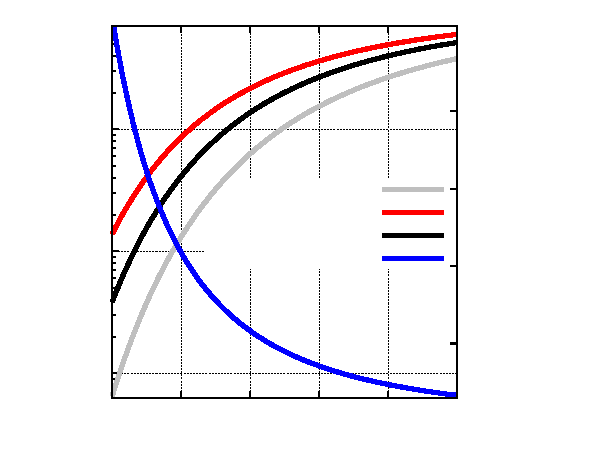
\includegraphics{EnergiesTransmissionCalibration}}%
    \gplfronttext
  \end{picture}%
\endgroup
}\label{fig:EnergiesTransmissionCalibration}}
		\subfloat[Calibrated sucrose concentration]{\resizebox{0.44\linewidth}{!}{% GNUPLOT: LaTeX picture with Postscript
\begingroup
  \makeatletter
  \providecommand\color[2][]{%
    \GenericError{(gnuplot) \space\space\space\@spaces}{%
      Package color not loaded in conjunction with
      terminal option `colourtext'%
    }{See the gnuplot documentation for explanation.%
    }{Either use 'blacktext' in gnuplot or load the package
      color.sty in LaTeX.}%
    \renewcommand\color[2][]{}%
  }%
  \providecommand\includegraphics[2][]{%
    \GenericError{(gnuplot) \space\space\space\@spaces}{%
      Package graphicx or graphics not loaded%
    }{See the gnuplot documentation for explanation.%
    }{The gnuplot epslatex terminal needs graphicx.sty or graphics.sty.}%
    \renewcommand\includegraphics[2][]{}%
  }%
  \providecommand\rotatebox[2]{#2}%
  \@ifundefined{ifGPcolor}{%
    \newif\ifGPcolor
    \GPcolortrue
  }{}%
  \@ifundefined{ifGPblacktext}{%
    \newif\ifGPblacktext
    \GPblacktextfalse
  }{}%
  % define a \g@addto@macro without @ in the name:
  \let\gplgaddtomacro\g@addto@macro
  % define empty templates for all commands taking text:
  \gdef\gplbacktext{}%
  \gdef\gplfronttext{}%
  \makeatother
  \ifGPblacktext
    % no textcolor at all
    \def\colorrgb#1{}%
    \def\colorgray#1{}%
  \else
    % gray or color?
    \ifGPcolor
      \def\colorrgb#1{\color[rgb]{#1}}%
      \def\colorgray#1{\color[gray]{#1}}%
      \expandafter\def\csname LTw\endcsname{\color{white}}%
      \expandafter\def\csname LTb\endcsname{\color{black}}%
      \expandafter\def\csname LTa\endcsname{\color{black}}%
      \expandafter\def\csname LT0\endcsname{\color[rgb]{1,0,0}}%
      \expandafter\def\csname LT1\endcsname{\color[rgb]{0,1,0}}%
      \expandafter\def\csname LT2\endcsname{\color[rgb]{0,0,1}}%
      \expandafter\def\csname LT3\endcsname{\color[rgb]{1,0,1}}%
      \expandafter\def\csname LT4\endcsname{\color[rgb]{0,1,1}}%
      \expandafter\def\csname LT5\endcsname{\color[rgb]{1,1,0}}%
      \expandafter\def\csname LT6\endcsname{\color[rgb]{0,0,0}}%
      \expandafter\def\csname LT7\endcsname{\color[rgb]{1,0.3,0}}%
      \expandafter\def\csname LT8\endcsname{\color[rgb]{0.5,0.5,0.5}}%
    \else
      % gray
      \def\colorrgb#1{\color{black}}%
      \def\colorgray#1{\color[gray]{#1}}%
      \expandafter\def\csname LTw\endcsname{\color{white}}%
      \expandafter\def\csname LTb\endcsname{\color{black}}%
      \expandafter\def\csname LTa\endcsname{\color{black}}%
      \expandafter\def\csname LT0\endcsname{\color{black}}%
      \expandafter\def\csname LT1\endcsname{\color{black}}%
      \expandafter\def\csname LT2\endcsname{\color{black}}%
      \expandafter\def\csname LT3\endcsname{\color{black}}%
      \expandafter\def\csname LT4\endcsname{\color{black}}%
      \expandafter\def\csname LT5\endcsname{\color{black}}%
      \expandafter\def\csname LT6\endcsname{\color{black}}%
      \expandafter\def\csname LT7\endcsname{\color{black}}%
      \expandafter\def\csname LT8\endcsname{\color{black}}%
    \fi
  \fi
  \setlength{\unitlength}{0.0500bp}%
  \begin{picture}(5668.00,4534.00)%
    \gplgaddtomacro\gplbacktext{%
      \csname LTb\endcsname%
      \put(814,942){\makebox(0,0)[r]{\strut{} 0}}%
      \csname LTb\endcsname%
      \put(814,1417){\makebox(0,0)[r]{\strut{} 10}}%
      \csname LTb\endcsname%
      \put(814,1892){\makebox(0,0)[r]{\strut{} 20}}%
      \csname LTb\endcsname%
      \put(814,2368){\makebox(0,0)[r]{\strut{} 30}}%
      \csname LTb\endcsname%
      \put(814,2843){\makebox(0,0)[r]{\strut{} 40}}%
      \csname LTb\endcsname%
      \put(814,3318){\makebox(0,0)[r]{\strut{} 50}}%
      \csname LTb\endcsname%
      \put(814,3794){\makebox(0,0)[r]{\strut{} 60}}%
      \csname LTb\endcsname%
      \put(814,4269){\makebox(0,0)[r]{\strut{} 70}}%
      \csname LTb\endcsname%
      \put(946,484){\makebox(0,0){\strut{} 0}}%
      \csname LTb\endcsname%
      \put(2027,484){\makebox(0,0){\strut{} 5}}%
      \csname LTb\endcsname%
      \put(3109,484){\makebox(0,0){\strut{} 10}}%
      \csname LTb\endcsname%
      \put(4190,484){\makebox(0,0){\strut{} 15}}%
      \csname LTb\endcsname%
      \put(5271,484){\makebox(0,0){\strut{} 20}}%
      \put(176,2486){\rotatebox{-270}{\makebox(0,0){\strut{}Sucrose Mass Fraction / $\%$}}}%
      \put(3108,154){\makebox(0,0){\strut{}Vertical Position / mm}}%
    }%
    \gplgaddtomacro\gplfronttext{%
      \csname LTb\endcsname%
      \put(4284,4096){\makebox(0,0)[r]{\strut{}5500 eV}}%
      \csname LTb\endcsname%
      \put(4284,3876){\makebox(0,0)[r]{\strut{}8000 eV}}%
      \csname LTb\endcsname%
      \put(4284,3656){\makebox(0,0)[r]{\strut{}10000 eV}}%
    }%
    \gplbacktext
    \put(0,0){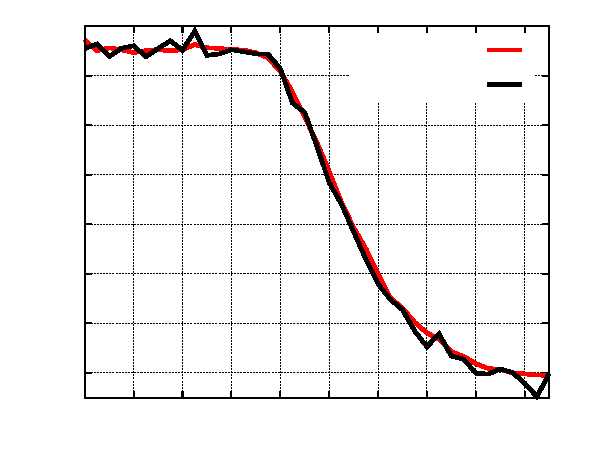
\includegraphics{SucroseTransmissionCalibration}}%
    \gplfronttext
  \end{picture}%
\endgroup
}\label{fig:SucroseTransmissionCalibration}}
	\caption{Statistics in the transmission measurement depending on the incoming energy. For lower energies, the transmission differences are larger and hence the statistics better. This was measured using only aqueous sucrose $65\%$ in plain water (no colloids on it) Nov 2014}
\end{figure}


\subsection{Limitations}
\subsubsection{Density range}
sucrose, fructose, iodixanol
\subsubsection{Challenges with different contrast agents}
Background subtraction, induced aggregation by heavy salts
\subsubsection{Comparison to other contrast variation scattering techinques}
SANS (deuterated water)
RSoXS in polymeric colloids (H.Abe 2006), Carbon K-edge

